\documentclass[12pt, a4paper]{article}
\title{Chapter 1}
\author{Maciej Harbuz}
\usepackage{amssymb}
\usepackage{amsmath}
\usepackage{tikz} 
\usepackage{import}
\usepackage{float}
\newcommand{\Mod}[1]{\ (\mathrm{mod}\ #1)}
\usetikzlibrary{automata, positioning, arrows}
\includeonly{chapter01-exercises-101-106.tex}
\tikzset{
    ->, % makes the edges directed
    every state/.style={thick, fill=gray!15}, % sets the properties for each ’state’ node
    node distance=2.5cm, % specifies the minimum distance between two nodes. Change if necessary.
    initial text=$ $, % sets the text that appears on the start arrow
    >=stealth, % makes the arrow heads bold
}

\begin{document}

\maketitle

\section{Exercises}
\begin{enumerate}

    \item[0.1]
Examine the following formal descriptions of sets so that you understand which members they contain. Write a short informal English description of each set.
\begin{enumerate}

\item 
$\{1, 3, 5, 7, \ldots \}$

Set of odd, natural numbers.
\item 
$\{x \ldots, -4, -2, 0, 2, 4 \ldots \}$

Set of even, integer numbers.
\item 
$\{n \mid n = 2m \text{for some \textit{m}} \in \mathbb{N} \}$

Set of even, natural numbers.
\item 
$\{n \mid n = 2m \text{for some \textit{m}} \in \mathbb{N}, \text{and} n = 3k \text{for some} k \in \mathbb{N} \}$

Set of even, natural numbers that are also multiples of 3.
\item 
$\{w \mid w  \text{is a string of \textit{0s} and \textit{1s} and \textit{w} equals the reverse of} w\}$

Set of strings of 0s and 1s that are palindroms 
\item $\{ n \mid n \text{is an integer and}  n = n+1\}$

Set of integers that are equal to their successor which is \textit{empty set}
\end{enumerate}

    \item[0.2]
Write  formal descriptions  of the following sets.

\begin{enumerate}
\item The set containing the numbers 1, 10, and 100

    $\{1, 10, 100\}$
\item The set containing all integers that are greater than 5
    
    $\{n \mid n > 5, n \in \mathbb{Z}\}$
\item  The set containing all natural numbers that are less than 5:

    $\{n \mid n < 5, n \in \mathbb{N}\}$
\item The set containing the string "aba":

    $\{"aba"\}$
\item The set containing the empty string:

    $\{\epsilon\}$
\item The set containing nothing at all:

    $\emptyset$
\end{enumerate}

    \item[0.3]

Let $A$ be the set $\{x,y,z\}$ and $B$ be the set $\{x,y\}$
\begin{enumerate}
\item Is $A$ a subset of $B$? ($A \subseteq B$) 

    No, $A$ is not a subset of $B$
\item Is $B$ a subset of $A$? ($B \subseteq A$) 

    Yes, $B$ is a subset of $A$
\item What is the union of $A$ and $B$? ($A \cup B$) 

    $\{x,y,z\} = A$
\item What is the intersection of $A$ and $B$? ($A \cap B$) 

    $\{x,y\} = B$
\item What is the cross product $A$ and $B$? ($A \times B$) 

    $\{(x,x), (x,y), (y,x), (y,y), (z,x), (z,y)\}$

\item What is the power set of $B$? 

$\mathcal{P}(B) = \{\emptyset, \{x\}, \{y\}, \{x,y\}\}$
\end{enumerate}

    \item[0.4]
If $A$ has  $a$  elements and  $B$  has  $b$  elements, how many elements are in  $A \times B$? 
Explain your answer.

The cross product of two sets $A$ and $B$ is the set of all possible ordered pairs of elements from $A$ and $B$. If $A$ has $a$ elements and $B$ has $b$ elements, then the cross product $A \times B$ will have $a \cdot b$ elements.

    \item[0.5]
If $C$ is a set with $c$ elements, how many elements are in the power set of $C$? 
Explain your answer.

The power set of a set $C$ is the set of all possible subsets of $C$. If $C$ has $c$ elements, then the power set of $C$ will have $2^c$ elements. Thats  because every element can be present or absent in every subset, so there are $2^c$ possible combinations of elements in the power set of $C$.

    \item[0.6]
Let X be the set $\{1, 2, 3, 4, 5\}$ and $Y$ be the set $\{6, 7, 8, 9, 10\}$. The unary function $f: X \to Y$ and the binary function $g: X \times Y \to Y$ are described in the following tables.

\begin{tabular}{ c | c }
    n & f(n) \\
    \hline
    1 & 6 \\
    2 & 7 \\
    3 & 6 \\
    4 & 7 \\
    5 & 6 \\
\end{tabular}
\begin{tabular}{ c | c | c | c | c | c }
    g(x,y) & 6 & 7 & 8 & 9 & 10 \\
    \hline
    1 & 10 & 10 & 10 & 10 & 10 \\
    2 & 7 & 8 & 9 & 10 & 6 \\
    3 & 7 & 7 & 8 & 8 & 9 \\
    4 & 9 & 8 & 7 & 6 & 10 \\
    5 & 6 & 6 & 6 & 6 & 6 \\
\end{tabular}
\begin{enumerate}
\item What is the value of f(2)? 

    $f(2) = 7$
\item What are the range and domain of f?
\begin{itemize}
    \item Range: $\{6, 7\}$
    \item Domain: $\{1, 2, 3, 4, 5\}$
\end{itemize}

\item What is the value of $g(2, 10)$?

    $g(2, 10) = 6$
\item What are the range and domain of g?
\begin{itemize}
    \item Range: $\{6, 7, 8, 9, 10\}$
    \item Domain: $\{1, 2, 3, 4, 5\}$
\end{itemize}

\item What is the value of $g(4, f(4))$?

    $g(4, f(4)) = 8$
\end{enumerate}

    \item[0.7]
For each part, give a relation that satisfies the condition.
\begin{enumerate}
    \item  Reflexive
    \footnote{Reflexive relation $R$ is when $\forall a \in A, (a, a) \in R$} and symmetric
    \footnote{Symmetric relation $R$ is when $\forall a, b \in A, (a, b) \in R \implies (b, a) \in R$} but not transitive.
    \item  Reflexive and transitive
    \footnote{Transitive relation $R$ is when $\forall a, b, c \in A, (a, b) \in R \land (b, c) \in R \implies (a, c) \in R$} but not symmetric.
    \item  Symmetric and transitive but not reflexive.
\end{enumerate}

\begin{enumerate}

    \item Reflexive and symmetric but not transitive example is be coworker relation on the set of people (let's assume that everybody is a coworker with themselves)
    \item Reflexive and transitive but not symmetric example is greater than or equal to relation on the set of natural numbers
    \item Symmetric and transitive but not reflexive example is the relation "is a sibling of" on the set of people
\end{enumerate}

    \item[0.8]
Consider the undirected graph $G = (V, E)$ where $V$, the set of nodes, is $\{1, 2, 3, 4\}$ and $E$, the set of edges, is $\{\{1, 2\}, \{2, 3\}, \{1, 3\}, \{2, 4\}, \{1, 4\}\}$. Draw the graph $G$. What are the degrees of each node? Indicate a path from node 3 to node 4 on your drawing of $G$.

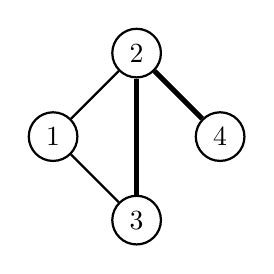
\begin{tikzpicture}[node distance={15mm}, thick, main/.style = {draw, circle}] 
\node[main] (1) {$1$}; 
\node[main] (2) [above right of=1] {$2$}; 
\node[main] (3) [below right of=1] {$3$}; 
\node[main] (4) [above right of=3] {$4$}; 
\draw[-] (1) -- (2); 
\draw[-] (1) -- (3); 
\draw[-, line width=1.8pt] (2) -- (3); 
\draw[-, line width=1.8pt] (2) -- (4); 
\end{tikzpicture} 

    \item[0.9]
Write a formal description of the following graph.

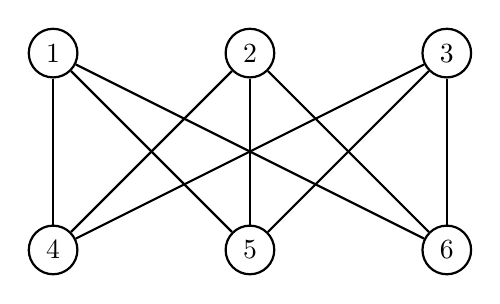
\begin{tikzpicture}[node distance={25mm}, thick, main/.style = {draw, circle}] 
    \node[main] (1) {$1$}; 
    \node[main] (2) [right of=1] {$2$}; 
    \node[main] (3) [right of=2] {$3$}; 
    \node[main] (4) [below of=1] {$4$}; 
    \node[main] (5) [right of=4] {$5$}; 
    \node[main] (6) [right of=5] {$6$}; 
    \draw[-] (1) -- (4); 
    \draw[-] (1) -- (5);
    \draw[-] (1) -- (6);
    \draw[-] (2) -- (4);
    \draw[-] (2) -- (5);
    \draw[-] (2) -- (6); 
    \draw[-] (3) -- (4);
    \draw[-] (3) -- (5);
    \draw[-] (3) -- (6); 
    \end{tikzpicture} 

$G = (V, E)$ where 

$V = \{1, 2, 3, 4, 5, 6\}$ and 

$E = \{\{1, 4\}, \{1, 5\}, \{1, 6\}, \{2, 4\}, \{2, 5\}, \{2, 6\}, \{3, 4\}, \{3, 5\}, \{3, 6\}\}$
\end{enumerate}


\begin{enumerate}

    \item[0.10]
Find the error in the following proof that $2 = 1$. 

Consider the equation $a = b$. Multiply both sides by a to obtain 
$a^2 = ab$. 
Subtract 
$b^2$ 
from both sides to get 
$a^2 - b^2 = ab - b^2$
. Now factor each side, 
$(a + b)(a - b) = b(a - b)$
, and divide each side by 
$(a - b)$ 
to get 
$a + b = b$
. Finally, let a and $b$ equal $1$, which shows that $2 = 1$.


We cannot divide each side of equation $(a + b)(a - b) = b(a - b)$ by $(a - b)$ because $a = b$ implies $a - b = 0$ and division by zero is undefined.

    \item[0.11]
Let $S(n) = 1 + 2 + \ldots + n$ be the sum of the first $n$ natural numbers, and let $C(n) = 1^3 + 2^3 + \ldots + n^3$ be the sum of the first n cubes. Prove the following equalities by induction on $n$, to arrive at the curious conclusion that $C(n) = S^2(n)$ for every $n$.

1. $S(n) = \frac{1}{2} n(n+1)$.

\textbf{Basis}
$ S(1) = 1 = \frac{1}{2} 1(1+1)$.

\textbf{Induction step}

$ S(k+1) = S(k) + (k+1) = \frac{1}{2} k(k+1) + (k+1) = \frac{1}{2} (k+1)(k+2)$.

2. $C(n) = \frac{1}{4}(n^4 + 2n^3 + n^2) = \frac{1}{4} n^2(n+1)^2$.

\textbf{Basis}

$ C(1) = 1 = \frac{1}{4} 1^2(1+1)^2$

\textbf{Induction step}

$ C(k+1) = C(k) + (k+1)^3 = \frac{1}{4} k^2(k+1)^2 + (k+1)^3 = \frac{1}{4} (k+1)^2(k+2)^2$.

The induction step is valid for both $S(n)$ and $C(n)$. 

Therefore, $C(n) = S^2(n)$ for every $n$.

$S^2(n)$ is $(\frac{1}{2} n(n+1))^2 = \frac{1}{4} n^2(n+1)^2$ which is equal to $C(n)$.

    \item[0.12]
Find the error in the following proof that all horses are the same color.

\textbf{CLAIM}: In any set of h horses, all horses are the same color.

\textbf{PROOF}: By induction on h.

\textbf{Basis}: 

For $h = 1$. In any set containing just one horse, all horses clearly are the same color.

\textbf{Induction step}

For $k >= 1$, assume that the claim is true for $h = k$ and prove that it is true for $h = k+1$. Take any set $H$ of $k+1$ horses. We show that all the horses in this set are the same color. Remove one horse from this set to obtain the set $H_1$ with just $k$ horses. By the induction hypothesis, all the horses in $H_1$ are the same color. Now replace the removed horse and remove a different one to obtain the set $H_2$. By the same argument, all the horses in $H_2$ are the same color. Therefore, all the horses in $H$ must be the same color, and the proof is complete.

The horse removed in the first step may have a different color than the horse removed in the second step. Therefore, the induction step is invalid.

\item[0.13]
Show that every graph with two or more nodes contains two nodes that have equal degrees.

A graph $G$ is a pair of sets $V$ and $E$ where the elements of the non empty set V are called the vertices and the elements of a possibly empty set E, called the edges, are unordered pairs of vertices.\footnote{https://www.quora.com/How-would-we-prove-that-every-graph-with-at-least-two-vertices-has-two-vertices-of-the-same-degree}

...

Depending on the cardinality of the set V graphs may be finite or infinite. I will only consider finite graphs.

Narrowing the scope further: I shall only consider graphs with no loops and with no multiple edges - in what follows a pair of vertices may be connected with at most one edge.

A vertex 
$v$
 is incident with an edge 
$e$
 if 
$v$
 is a terminal point of 
$e$
. As such, the degree of a vertex 
$v$
 is the number of edges incident with 
$v$
. Intuitively - say, as a vertex I’m a city: the number of distinct roads that emanate from or lead into me is my degree.

Further, since our edge must connect exactly two distinct vertices, 
$a$
 and 
$b$
, it follows that when we count the degree of a connected vertex, 
$a$
 or 
$b$
, we “overcount its edge” (loosely speaking) - that edge contributes 
$1$
 toward the total degree of $a$ and it also contributes $1$ toward the total degree of $b$.
Therefore, the sum of degrees $d_{i}$ (some of which may be zero) of $n$ vertices of a graph must be an even number (in $e$ - the number of edges in a graph):

$$\sum^{n}_{i=1}=1 d_{i}=2e$$

Now onto the theorem - proof by contradiction.

Observe that if the number of vertices in our graph is $n$ then the largest degree of any vertex in such a graph must be strictly less then $n$:

$$max d_{i} \leq n-1$$
for any 
i
. Why is that? By contradiction. Recall my roads leaving a city analogy - a road emanating from a given (and fixed) city has only and at most 
n - 1
 other cities to go to since:

no loops and
no multiple roads to the same city
are allowed.

Next, assume that, contrary to the conclusion, each and every vertex has a distinct degree. Therefore, our only choices (for these degrees) are:

$D={0,1,2,3,\ldots ,n-1}$

But our graph can not have two vertices with degrees 
$0$
 and 
$n-1$
 simultaneously.

Why is that?

By contradiction - assume that a graph has a vertex $v$
 with degree 
n-1
 . Then 
v
 must find exactly 
n-1
 distinct cities on the other side. Therefore, in that case a vertex with degree 
0
 can not exist.

Therefore, our set of choices (3) splits into two: either:

$D = \{ 1 , 2 , 3 , 4 , \ldots ,n - 1 \}$

or:

$D = \{ 0, 1, 2, 3, \ldots , n-2\}$


But in either case the cardinality of $D$ is $n-1$:

$|D|=n-1$

Therefore, we have to distribute $n$ vertices over $n-1$ degrees and by pigeonhole principle, since we have more vertices (pigeons) than degrees (pigeonholes):

at least two vertices must share the same degree

which amounts to a contradiction - our initial assumption that all the degrees are distinct was false. Therefore, if our graph has at least two vertices then at least two of them have the same degree.

\item[0.14]
Ramsey's theorem. 

Let $G$ be a graph. A clique in $G$ is a subgraph in which every two nodes are connected by an edge. An anti-clique, also called an independent set, is a subgraph in which every two nodes are not connected by an edge. Show that every graph with $n$ nodes contains either a clique or an anti-clique with at least $\frac{1}{2} log_2(n)$ nodes.


\item[0.15]
Use Theorem 0.25 to derive a formula for calculating the size of the monthly payment for a mortgage in terms of the principal P, the interest rate I, and the number of payments t. Assume that after t payments have been made, the loan amount is reduced to 0. Use the formula to calculate the dollar amount of each monthly payment for a 30-year mortgage with 360 monthly payments on an initial loan amount of \$100,000 with a 5% annual interest rate.


\textbf{Theorem 0.25}

$\forall t \geq 0$


$P_t=PM^t-Y\frac{M^t-1}{M-1}$
\end{enumerate}
\begin{enumerate}

    \item[1.1]
          The following are the state diagrams of two DFAs, $M_1$ and $M_2$. Answer the following questions about each of these machines.

          \begin{figure}[H]
              \centering
              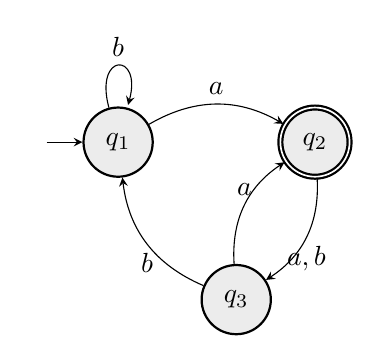
\begin{tikzpicture}
                  \node[state, initial] (q1) {$q_1$};
                  \node[state, accepting, right of=q1] (q2) {$q_2$};
                  \node[state] at (1.5, -2) (q3) {$q_3$};
                  \draw (q1) edge[loop above] node{$b$} (q1)
                  (q1) edge[bend left, above] node{$a$} (q2)
                  (q2) edge[bend left, below] node{$a,b$} (q3)
                  (q3) edge[bend left, above] node{$a$} (q2)
                  (q3) edge[bend left, below] node{$b$} (q1);
              \end{tikzpicture}
              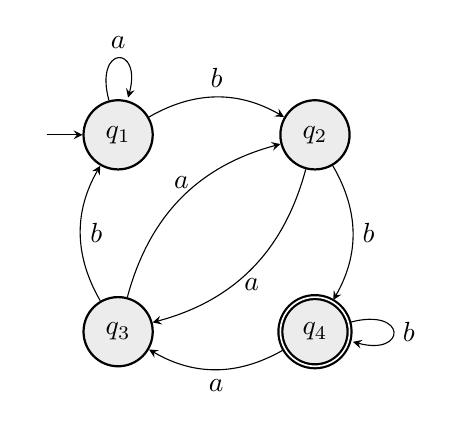
\begin{tikzpicture}
                  \node[state, initial] (q1) {$q_1$};
                  \node[state, right of=q1] (q2) {$q_2$};
                  \node[state, below of=q1] (q3) {$q_3$};
                  \node[state, accepting, below of=q2] (q4) {$q_4$};
                  \draw (q1) edge[loop above] node{$a$} (q1)
                  (q1) edge[bend left, above] node{$b$} (q2)
                  (q2) edge[bend left, below] node{$a$} (q3)
                  (q2) edge[bend left, right] node{$b$} (q4)
                  (q3) edge[bend left, above] node{$a$} (q2)
                  (q3) edge[bend left, right] node{$b$} (q1)
                  (q4) edge[bend left, below] node{$a$} (q3)
                  (q4) edge[loop right] node{$b$} (q4);
              \end{tikzpicture}
              \caption{$M_1$ and $M_2$}
          \end{figure}

          \begin{enumerate}
              \item What is the start state?

                    $M_1: q_1$

                    $M_2: q_1$

              \item What is the set of accept states?

                    $M_1: \{q_2\}$

                    $M_2: \{q_4\}$
              \item What sequence of states does the machine go through on input $aabb$?

                    $M_1: q_1 \rightarrow q_2 \rightarrow q_3 \rightarrow q_1 \rightarrow q_1$

                    $M_2: q_1 \rightarrow q_2 \rightarrow q_4 \rightarrow q_4 \rightarrow q_4$
              \item Does the machine accept the string $aabb$?

                    $M_1:$ No

                    $M_2:$ Yes
              \item Does the machine accept the string $\epsilon$?

                    $M_1:$ No

                    $M_2:$ No
          \end{enumerate}

    \item[1.2]

          Give the formal description of the machines $M_1$ and $M_2$ pictured in Exercise 1.1.

          $M_1 = (Q, \Sigma_1, \delta_1, q_1, \{q_2\})$

          $Q = \{q_1, q_2, q_3\}$

          $\Sigma_1 = \{a, b\}$

          $\delta_1 = \{((q_1, a), q_2), ((q_1, b), q_1), ((q_2, a), q_3), ((q_2, b), q_3), ((q_3, a), q_2), ((q_3, b), q_1)\}$\\

          $M_2 = (Q, \Sigma_2, \delta_2, q_1, \{q_4\})$

          $Q = \{q_1, q_2, q_3, q_4\}$

          $\Sigma_2 = \{a, b\}$

          $\delta_2 = \{((q_1, a), q_1), ((q_1, b), q_2), ((q_2, a), q_3), ((q_2, b), q_4),$\\
          .\,\,\,\qquad$((q_3, a), q_2), ((q_3, b), q_1), ((q_4, a), q_3), ((q_4, b), q_4)\}$

    \item[1.3]

          The formal description of a DFA $M$ is $\{q_1,q_2,q_3,q_4,q_5\},\{u,d\},\sigma,q_3,\{q_3\}$, where $\sigma$ is given by the following table. Give the state diagram of this machine.

          \begin{center}


              \begin{tabular}{ c | c c }
                        & $u$   & $d$   \\
                  \hline
                  $q_1$ & $q_1$ & $q_2$ \\
                  $q_2$ & $q_1$ & $q_3$ \\
                  $q_3$ & $q_2$ & $q_4$ \\
                  $q_4$ & $q_3$ & $q_5$ \\
                  $q_5$ & $q_4$ & $q_5$ \\
              \end{tabular}
          \end{center}

          \begin{figure}[H]
              \centering
              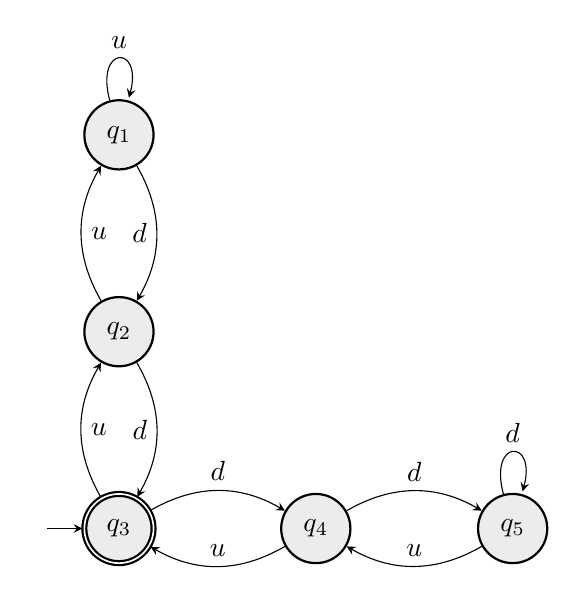
\begin{tikzpicture}
                  \node[state] (q1) {$q_1$};
                  \node[state, below of=q1] (q2) {$q_2$};
                  \node[state, accepting, initial, below of=q2] (q3) {$q_3$};
                  \node[state, right of=q3] (q4) {$q_4$};
                  \node[state, right of=q4] (q5) {$q_5$};
                  \draw (q1) edge[loop above] node{$u$} (q1)
                  (q1) edge[bend left, left] node{$d$} (q2)
                  (q2) edge[bend left, right] node{$u$} (q1)
                  (q2) edge[bend left, left] node{$d$} (q3)
                  (q3) edge[bend left, right] node{$u$} (q2)
                  (q3) edge[bend left, above] node{$d$} (q4)
                  (q4) edge[bend left, above] node{$u$} (q3)
                  (q4) edge[bend left, above] node{$d$} (q5)
                  (q5) edge[loop above] node{$d$} (q5)
                  (q5) edge[bend left, above] node{$u$} (q4);
              \end{tikzpicture}
          \end{figure}

    \item[1.4]
          Each of the following languages is the intersection of two simpler languages. In each part, construct DFAs for the simpler languages,then combine them using the construction discussed in footnote 3 (page 46) to give the state diagram of a DFA for the language given. In all parts, $\Sigma=\{a,b\}$.
          \begin{enumerate}
              \item $\{w|w~\text{has at least three }a\text{’s and at least two }b\text{’s}\}$

                    $DFA_1$ for at least three $a$'s:

                    \begin{figure}[H]
                        \centering
                        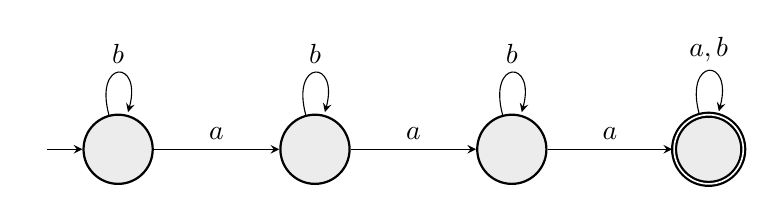
\begin{tikzpicture}
                            \node[state, initial] (q1) {};
                            \node[state, right of=q1] (q2) {};
                            \node[state, right of=q2] (q3) {};
                            \node[state, right of=q3, accepting] (q4) {};
                            \draw (q1) edge[loop above] node{$b$} (q1)
                            (q2) edge[loop above] node{$b$} (q2)
                            (q3) edge[loop above] node{$b$} (q3)
                            (q4) edge[loop above] node{$a,b$} (q4)
                            (q1) edge[left, above] node{$a$} (q2)
                            (q2) edge[left, above] node{$a$} (q3)
                            (q3) edge[left, above] node{$a$} (q4);
                        \end{tikzpicture}
                    \end{figure}

                    $DFA_2$ for at least two $b$'s:

                    \begin{figure}[H]
                        \centering
                        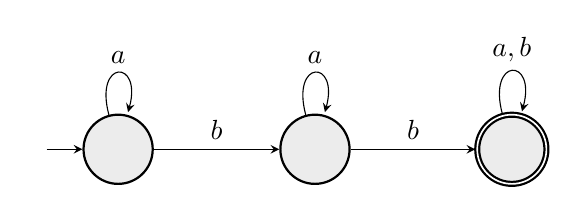
\begin{tikzpicture}
                            \node[state, initial] (q1) {};
                            \node[state, right of=q1] (q2) {};
                            \node[state, right of=q2, accepting] (q3) {};
                            \draw (q1) edge[loop above] node{$a$} (q1)
                            (q2) edge[loop above] node{$a$} (q2)
                            (q3) edge[loop above] node{$a,b$} (q3)
                            (q1) edge[left, above] node{$b$} (q2)
                            (q2) edge[left, above] node{$b$} (q3);
                        \end{tikzpicture}
                    \end{figure}

                    $DFA$ for at least three $a$'s and at least two $b$'s:

                    \begin{figure}[H]
                        \centering
                        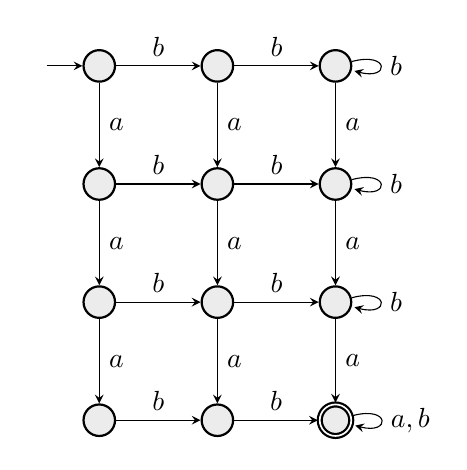
\begin{tikzpicture}[
                                styleSmall/.style={minimum size=4mm},
                                node distance=1.5cm,
                            ]
                            \node[state, initial, styleSmall] (q11) {};
                            \node[state, right of=q11, styleSmall] (q12) {};
                            \node[state, right of=q12, styleSmall] (q13) {};
                            \node[state, below of=q11, styleSmall] (q21) {};
                            \node[state, below of=q12, styleSmall] (q22) {};
                            \node[state, below of=q13, styleSmall] (q23) {};
                            \node[state, below of=q21, styleSmall] (q31) {};
                            \node[state, below of=q22, styleSmall] (q32) {};
                            \node[state, below of=q23, styleSmall] (q33) {};
                            \node[state, below of=q31, styleSmall] (q41) {};
                            \node[state, below of=q32, styleSmall] (q42) {};
                            \node[state, below of=q33, styleSmall, accepting] (q43) {};
                            \draw
                            (q13) edge[loop right] node{$b$} (q13)

                            (q11) edge[left, above] node{$b$} (q12)
                            (q12) edge[left, above] node{$b$} (q13)
                            (q23) edge[loop right] node{$b$} (q23)
                            (q21) edge[left, above] node{$b$} (q22)
                            (q22) edge[left, above] node{$b$} (q23)
                            (q33) edge[loop right] node{$b$} (q33)
                            (q31) edge[left, above] node{$b$} (q32)
                            (q32) edge[left, above] node{$b$} (q33)
                            (q43) edge[loop right] node{$a,b$} (q43)
                            (q41) edge[left, above] node{$b$} (q42)
                            (q42) edge[left, above] node{$b$} (q43)

                            (q11) edge[left, right] node{$a$} (q21)
                            (q12) edge[left, right] node{$a$} (q22)
                            (q13) edge[left, right] node{$a$} (q23)
                            (q21) edge[left, right] node{$a$} (q31)
                            (q22) edge[left, right] node{$a$} (q32)
                            (q23) edge[left, right] node{$a$} (q33)
                            (q31) edge[left, right] node{$a$} (q41)
                            (q32) edge[left, right] node{$a$} (q42)
                            (q33) edge[left, right] node{$a$} (q43);
                        \end{tikzpicture}
                    \end{figure}

              \item $\{w|w~\text{has exactly two }a\text{’s and at least two }b\text{’s}\}$

                    $DFA_1$ for exactly two $a$'s:

                    \begin{figure}[H]
                        \centering
                        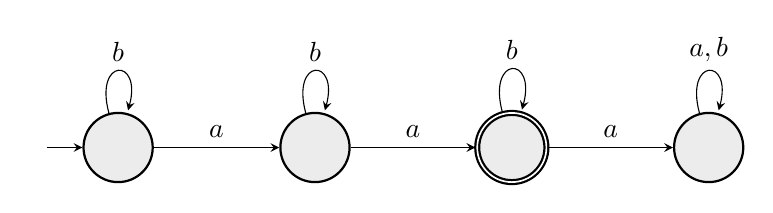
\begin{tikzpicture}
                            \node[state, initial] (q1) {};
                            \node[state, right of=q1] (q2) {};
                            \node[state, right of=q2, accepting] (q3) {};
                            \node[state, right of=q3] (q4) {};
                            \draw (q1) edge[loop above] node{$b$} (q1)
                            (q2) edge[loop above] node{$b$} (q2)
                            (q3) edge[loop above] node{$b$} (q3)
                            (q4) edge[loop above] node{$a,b$} (q4)
                            (q1) edge[left, above] node{$a$} (q2)
                            (q2) edge[left, above] node{$a$} (q3)
                            (q3) edge[left, above] node{$a$} (q4);
                        \end{tikzpicture}
                    \end{figure}

                    $DFA_2$ for at least two $b$'s:

                    \begin{figure}[H]
                        \centering
                        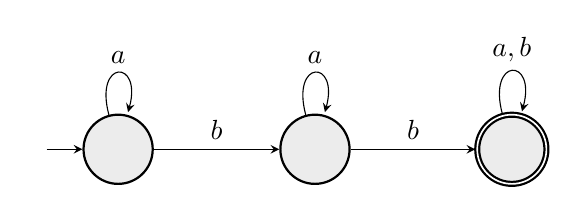
\begin{tikzpicture}
                            \node[state, initial] (q1) {};
                            \node[state, right of=q1] (q2) {};
                            \node[state, right of=q2, accepting] (q3) {};
                            \draw (q1) edge[loop above] node{$a$} (q1)
                            (q2) edge[loop above] node{$a$} (q2)
                            (q3) edge[loop above] node{$a,b$} (q3)
                            (q1) edge[left, above] node{$b$} (q2)
                            (q2) edge[left, above] node{$b$} (q3);
                        \end{tikzpicture}
                    \end{figure}

                    $DFA$ for exactly two $a$'s and at least two $b$'s:

                    \begin{figure}[H]
                        \centering
                        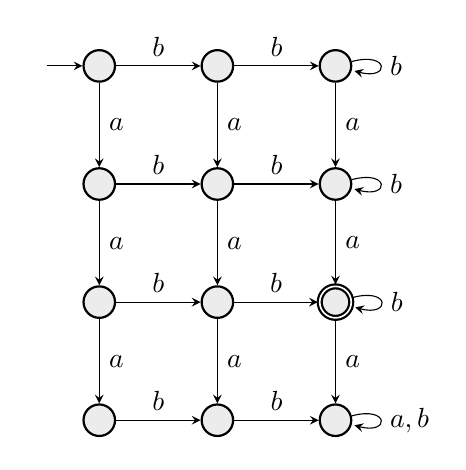
\begin{tikzpicture}[
                                styleSmall/.style={minimum size=4mm},
                                node distance=1.5cm,
                            ]
                            \node[state, initial, styleSmall] (q11) {};
                            \node[state, right of=q11, styleSmall] (q12) {};
                            \node[state, right of=q12, styleSmall] (q13) {};
                            \node[state, below of=q11, styleSmall] (q21) {};
                            \node[state, below of=q12, styleSmall] (q22) {};
                            \node[state, below of=q13, styleSmall] (q23) {};
                            \node[state, below of=q21, styleSmall] (q31) {};
                            \node[state, below of=q22, styleSmall] (q32) {};
                            \node[state, below of=q23, styleSmall, accepting] (q33) {};
                            \node[state, below of=q31, styleSmall] (q41) {};
                            \node[state, below of=q32, styleSmall] (q42) {};
                            \node[state, below of=q33, styleSmall] (q43) {};
                            \draw
                            (q13) edge[loop right] node{$b$} (q13)
                            (q11) edge[left, above] node{$b$} (q12)
                            (q12) edge[left, above] node{$b$} (q13)
                            (q23) edge[loop right] node{$b$} (q23)
                            (q21) edge[left, above] node{$b$} (q22)
                            (q22) edge[left, above] node{$b$} (q23)
                            (q33) edge[loop right] node{$b$} (q33)
                            (q31) edge[left, above] node{$b$} (q32)
                            (q32) edge[left, above] node{$b$} (q33)
                            (q43) edge[loop right] node{$a,b$} (q43)
                            (q41) edge[left, above] node{$b$} (q42)
                            (q42) edge[left, above] node{$b$} (q43)

                            (q11) edge[left, right] node{$a$} (q21)
                            (q12) edge[left, right] node{$a$} (q22)
                            (q13) edge[left, right] node{$a$} (q23)
                            (q21) edge[left, right] node{$a$} (q31)
                            (q22) edge[left, right] node{$a$} (q32)
                            (q23) edge[left, right] node{$a$} (q33)
                            (q31) edge[left, right] node{$a$} (q41)
                            (q32) edge[left, right] node{$a$} (q42)
                            (q33) edge[left, right] node{$a$} (q43);
                        \end{tikzpicture}
                    \end{figure}

              \item $\{w|w~\text{has an even number of }a\text{’s and one or two }b\text{’s}\}$

                    $DFA_1$ for an even number of $a$'s:

                    \begin{figure}[H]
                        \centering
                        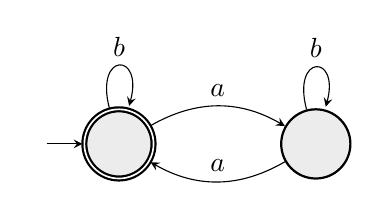
\begin{tikzpicture}
                            \node[state, initial, accepting] (q1) {};
                            \node[state, right of=q1] (q2) {};
                            \draw (q1) edge[loop above] node{$b$} (q1)
                            (q2) edge[loop above] node{$b$} (q2)
                            (q1) edge[bend left, above] node{$a$} (q2)
                            (q2) edge[bend left, above] node{$a$} (q1);
                        \end{tikzpicture}
                    \end{figure}

                    $DFA_2$ for one or two $b$'s:

                    \begin{figure}[H]
                        \centering
                        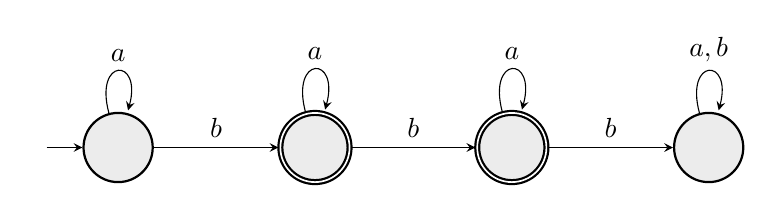
\begin{tikzpicture}
                            \node[state, initial] (q1) {};
                            \node[state, right of=q1, accepting] (q2) {};
                            \node[state, right of=q2, accepting] (q3) {};
                            \node[state, right of=q3] (q4) {};
                            \draw (q1) edge[loop above] node{$a$} (q1)
                            (q2) edge[loop above] node{$a$} (q2)
                            (q3) edge[loop above] node{$a$} (q3)
                            (q4) edge[loop above] node{$a,b$} (q4)
                            (q1) edge[left, above] node{$b$} (q2)
                            (q2) edge[left, above] node{$b$} (q3)
                            (q3) edge[left, above] node{$b$} (q4);
                        \end{tikzpicture}
                    \end{figure}

                    $DFA$ for an even number of $a$'s and one or two $b$'s:

                    \begin{figure}[H]
                        \centering
                        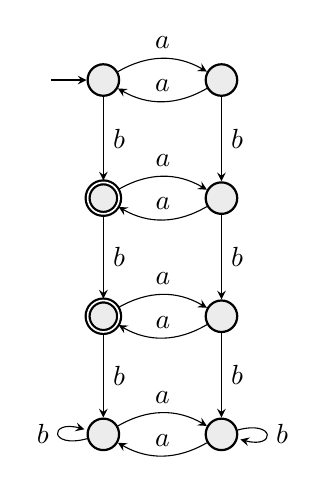
\begin{tikzpicture}[
                                styleSmall/.style={minimum size=4mm},
                                node distance=1.5cm,
                            ]
                            \node[state, initial, styleSmall] (q11) {};
                            \node[state, right of=q11, styleSmall] (q12) {};
                            \node[state, below of=q11, styleSmall, accepting] (q21) {};
                            \node[state, below of=q12, styleSmall] (q22) {};
                            \node[state, below of=q21, styleSmall, accepting] (q31) {};
                            \node[state, below of=q22, styleSmall] (q32) {};
                            \node[state, below of=q31, styleSmall] (q41) {};
                            \node[state, below of=q32, styleSmall] (q42) {};
                            \draw
                            (q11) edge[bend left, above] node{$a$} (q12)
                            (q12) edge[bend left, above] node{$a$} (q11)
                            (q21) edge[bend left, above] node{$a$} (q22)
                            (q22) edge[bend left, above] node{$a$} (q21)
                            (q31) edge[bend left, above] node{$a$} (q32)
                            (q32) edge[bend left, above] node{$a$} (q31)
                            (q41) edge[bend left, above] node{$a$} (q42)
                            (q42) edge[bend left, above] node{$a$} (q41)

                            (q41) edge[loop left] node{$b$} (q41)
                            (q42) edge[loop right] node{$b$} (q42)

                            (q11) edge[left, right] node{$b$} (q21)
                            (q12) edge[left, right] node{$b$} (q22)
                            (q21) edge[left, right] node{$b$} (q31)
                            (q22) edge[left, right] node{$b$} (q32)
                            (q31) edge[left, right] node{$b$} (q41)
                            (q32) edge[left, right] node{$b$} (q42);
                        \end{tikzpicture}
                    \end{figure}


              \item $\{w|w~\text{has an even number of }a\text{’s and each }a\text{ is followed by at least one }b\}$

                    $DFA_1$ for an even number of $a$'s:

                    \begin{figure}[H]
                        \centering
                        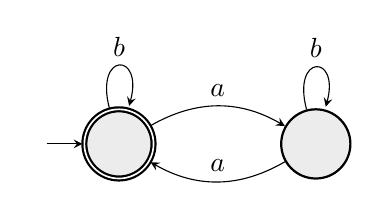
\begin{tikzpicture}
                            \node[state, initial, accepting] (q1) {};
                            \node[state, right of=q1] (q2) {};
                            \draw (q1) edge[loop above] node{$b$} (q1)
                            (q2) edge[loop above] node{$b$} (q2)
                            (q1) edge[bend left, above] node{$a$} (q2)
                            (q2) edge[bend left, above] node{$a$} (q1);
                        \end{tikzpicture}
                    \end{figure}

                    $DFA_2$ for each $a$ is followed by at least one $b$:

                    \begin{figure}[H]
                        \centering
                        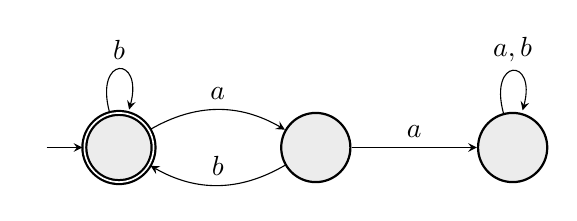
\begin{tikzpicture}
                            \node[state, initial, accepting] (q1) {};
                            \node[state, right of=q1] (q2) {};
                            \node[state, right of=q2] (q3) {};
                            \draw (q1) edge[loop above] node{$b$} (q1)
                            (q3) edge[loop above] node{$a,b$} (q3)
                            (q1) edge[bend left, above] node{$a$} (q2)
                            (q2) edge[bend left, above] node{$b$} (q1)
                            (q2) edge[left, above] node{$a$} (q3);
                        \end{tikzpicture}
                    \end{figure}

              \item $\{w|w~\text{starts with an }a\text{ and has at most one }b\}$

                    $DFA_1$ for starts with an $a$:

                    \begin{figure}[H]
                        \centering
                        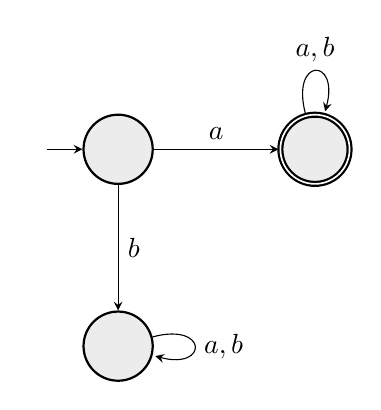
\begin{tikzpicture}
                            \node[state, initial] (q1) {};
                            \node[state, right of=q1, accepting] (q2) {};
                            \node[state, below of=q1 ] (q3) {};
                            \draw
                            (q3) edge[loop right] node{$a,b$} (q3)
                            (q2) edge[loop above] node{$a,b$} (q2)
                            (q1) edge[above] node{$a$} (q2)
                            (q1) edge[right] node{$b$} (q3);
                        \end{tikzpicture}
                    \end{figure}

                    $DFA_2$ for has at most one $b$:

                    \begin{figure}[H]
                        \centering
                        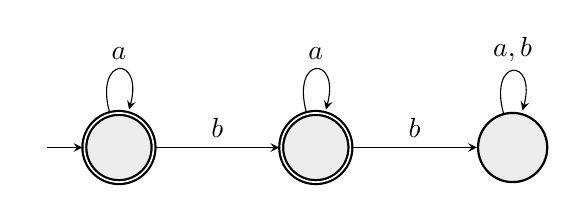
\begin{tikzpicture}
                            \node[state, initial, accepting] (q1) {};
                            \node[state, right of=q1, accepting] (q2) {};
                            \node[state, right of=q2] (q3) {};
                            \draw (q1) edge[loop above] node{$a$} (q1)
                            (q2) edge[loop above] node{$a$} (q2)
                            (q3) edge[loop above] node{$a,b$} (q3)
                            (q1) edge[left, above] node{$b$} (q2)
                            (q2) edge[left, above] node{$b$} (q3);
                        \end{tikzpicture}
                    \end{figure}

              \item $\{w|w~\text{has an odd number of }a\text{’s and ends with a }b\}$

                    $DFA_1$ for an odd number of $a$'s:

                    \begin{figure}[H]
                        \centering
                        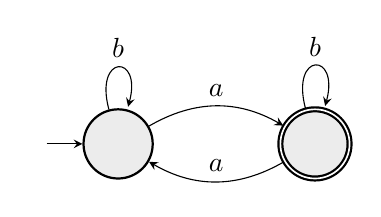
\begin{tikzpicture}
                            \node[state, initial] (q1) {};
                            \node[state, right of=q1, accepting] (q2) {};
                            \draw (q1) edge[loop above] node{$b$} (q1)
                            (q2) edge[loop above] node{$b$} (q2)
                            (q1) edge[bend left, above] node{$a$} (q2)
                            (q2) edge[bend left, above] node{$a$} (q1);
                        \end{tikzpicture}
                    \end{figure}

                    $DFA_2$ for ends with a $b$:

                    \begin{figure}[H]
                        \centering
                        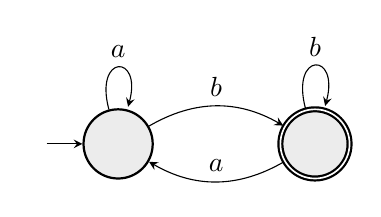
\begin{tikzpicture}
                            \node[state, initial] (q1) {};
                            \node[state, right of=q1, accepting] (q2) {};
                            \draw (q1) edge[loop above] node{$a$} (q1)
                            (q2) edge[loop above] node{$b$} (q2)
                            (q1) edge[bend left, above] node{$b$} (q2)
                            (q2) edge[bend left, above] node{$a$} (q1);
                        \end{tikzpicture}
                    \end{figure}

              \item $\{w|w~\text{has even length and an odd number of }a\text{’s}\}$

                    $DFA_1$ for even length:

                    \begin{figure}[H]
                        \centering
                        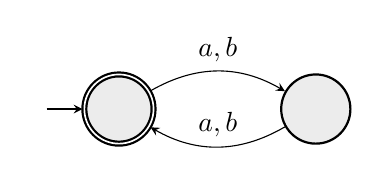
\begin{tikzpicture}
                            \node[state, initial, accepting] (q1) {};
                            \node[state, right of=q1] (q2) {};
                            \draw
                            (q1) edge[bend left, above] node{$a,b$} (q2)
                            (q2) edge[bend left, above] node{$a,b$} (q1);
                        \end{tikzpicture}
                    \end{figure}

                    $DFA_2$ for an odd number of $a$'s:

                    \begin{figure}[H]
                        \centering
                        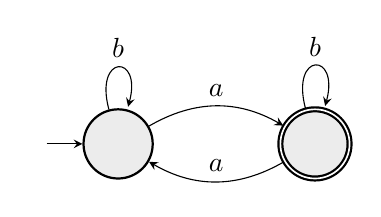
\begin{tikzpicture}
                            \node[state, initial] (q1) {};
                            \node[state, right of=q1, accepting] (q2) {};
                            \draw (q1) edge[loop above] node{$b$} (q1)
                            (q2) edge[loop above] node{$b$} (q2)
                            (q1) edge[bend left, above] node{$a$} (q2)
                            (q2) edge[bend left, above] node{$a$} (q1);
                        \end{tikzpicture}
                    \end{figure}

          \end{enumerate}

    \item[1.5]
          Each of the following languages is the complement of a simpler language. In each part, construct a DFA for the simpler language, then use it to give the state diagram of a DFA for the language given. In all parts, $\Sigma=\{a,b\}$.
          \begin{enumerate}
              \item $A = \{w|w~\text{does not contain the substring }ab\}$

                    $\overline{A} = \{w|w~\text{contains the substring }ab\}$
                    \begin{figure}[H]
                        \centering
                        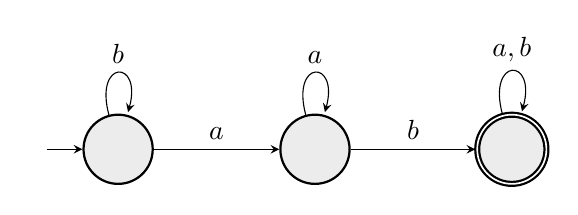
\begin{tikzpicture}
                            \node[state, initial] (q1) {};
                            \node[state, right of=q1] (q2) {};
                            \node[state, accepting, right of=q2] (q3) {};
                            \draw (q1) edge[left, above] node{$a$} (q2)
                            (q1) edge[loop above] node{$b$} (q1)
                            (q2) edge[left, above] node{$b$} (q3)
                            (q2) edge[loop above] node{$a$} (q2)
                            (q3) edge[loop above] node{$a,b$} (q3);
                        \end{tikzpicture}
                        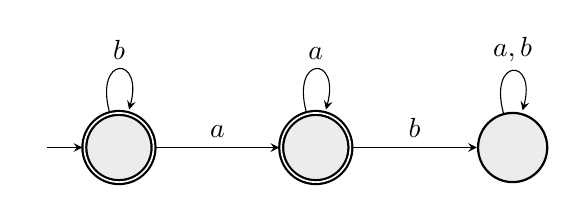
\begin{tikzpicture}
                            \node[state, accepting, initial] (q1) {};
                            \node[state, accepting, right of=q1] (q2) {};
                            \node[state, right of=q2] (q3) {};
                            \draw (q1) edge[left, above] node{$a$} (q2)
                            (q1) edge[loop above] node{$b$} (q1)
                            (q2) edge[left, above] node{$b$} (q3)
                            (q2) edge[loop above] node{$a$} (q2)
                            (q3) edge[loop above] node{$a,b$} (q3);
                        \end{tikzpicture}
                        \caption{$\overline{A}$ and $A$}
                    \end{figure}
              \item $B = \{w|w~\text{does notcontain the substring }baba\}$

                    $\overline{B} = \{w|w~\text{contains the substring }baba\}$
                    \begin{figure}[H]
                        \centering
                        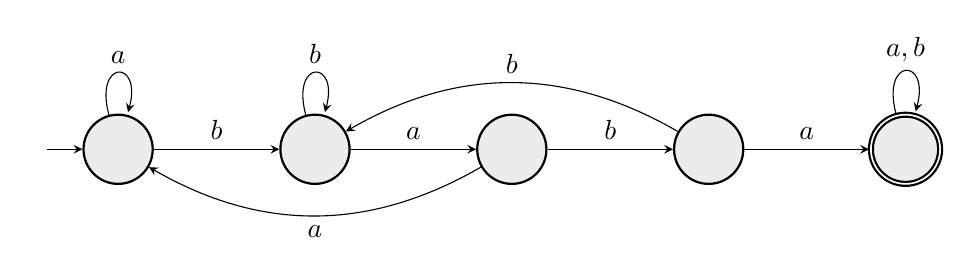
\begin{tikzpicture}
                            \node[state, initial] (q1) {};
                            \node[state, right of=q1] (q2) {};
                            \node[state, right of=q2] (q3) {};
                            \node[state, right of=q3] (q4) {};
                            \node[state, accepting, right of=q4] (q5) {};
                            \draw (q1) edge[left, above] node{$b$} (q2)
                            (q1) edge[loop above] node{$a$} (q1)
                            (q2) edge[left, above] node{$a$} (q3)
                            (q2) edge[loop above] node{$b$} (q2)
                            (q3) edge[left, above] node{$b$} (q4)
                            (q3) edge[bend left, below] node{$a$} (q1)
                            (q4) edge[bend right, above] node{$b$} (q2)
                            (q4) edge[left, above] node{$a$} (q5)
                            (q5) edge[loop above] node{$a,b$} (q5);
                        \end{tikzpicture}
                        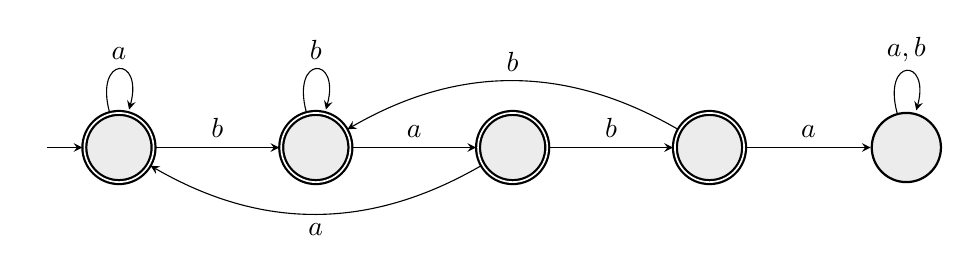
\begin{tikzpicture}
                            \node[state, accepting, initial] (q1) {};
                            \node[state, accepting, right of=q1] (q2) {};
                            \node[state, accepting, right of=q2] (q3) {};
                            \node[state, accepting, right of=q3] (q4) {};
                            \node[state, right of=q4] (q5) {};
                            \draw (q1) edge[left, above] node{$b$} (q2)
                            (q1) edge[loop above] node{$a$} (q1)
                            (q2) edge[left, above] node{$a$} (q3)
                            (q2) edge[loop above] node{$b$} (q2)
                            (q3) edge[left, above] node{$b$} (q4)
                            (q3) edge[bend left, below] node{$a$} (q1)
                            (q4) edge[bend right, above] node{$b$} (q2)
                            (q4) edge[left, above] node{$a$} (q5)
                            (q5) edge[loop above] node{$a,b$} (q5);
                        \end{tikzpicture}
                        \caption{$\overline{B}$ and $B$}
                    \end{figure}

              \item $C =\{w|w~\text{contains neither the substrings }ab\text{ nor }ba\}$

                    $\overline{C} = \{w|w~\text{contains the substring }ab\text{ or }ba\}$
                    \begin{figure}[H]
                        \centering
                        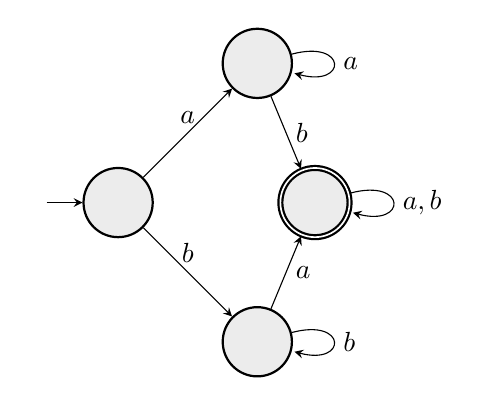
\begin{tikzpicture}
                            \node[state, initial] (q1) {};
                            \node[state, above right of=q1] (q2) {};
                            \node[state, below right of=q1] (q3) {};
                            \node[state, accepting, right of=q1] (q4) {};
                            \draw (q1) edge[left, above] node{$a$} (q2)
                            (q1) edge[left, above] node{$b$} (q3)
                            (q2) edge[right] node{$b$} (q4)
                            (q2) edge[loop right] node{$a$} (q2)
                            (q3) edge[right] node{$a$} (q4)
                            (q3) edge[loop right] node{$b$} (q3)
                            (q4) edge[loop right] node{$a,b$} (q4);
                        \end{tikzpicture}
                        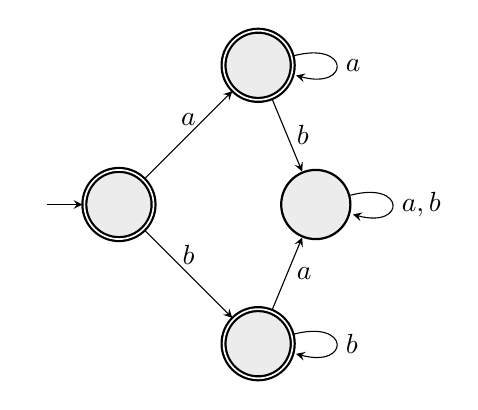
\begin{tikzpicture}
                            \node[state, accepting, initial] (q1) {};
                            \node[state, accepting, above right of=q1] (q2) {};
                            \node[state, accepting, below right of=q1] (q3) {};
                            \node[state, right of=q1] (q4) {};
                            \draw (q1) edge[left, above] node{$a$} (q2)
                            (q1) edge[left, above] node{$b$} (q3)
                            (q2) edge[right] node{$b$} (q4)
                            (q2) edge[loop right] node{$a$} (q2)
                            (q3) edge[right] node{$a$} (q4)
                            (q3) edge[loop right] node{$b$} (q3)
                            (q4) edge[loop right] node{$a,b$} (q4);
                        \end{tikzpicture}
                        \caption{$\overline{C}$ and $C$}
                    \end{figure}
              \item $D = \{w|w~\text{is any string not in }a^{\ast}b^{\ast}\}$

                    $\overline{D} = \{w|w~\text{is any string in }a^{\ast}b^{\ast}\}$
                    \begin{figure}[H]
                        \centering
                        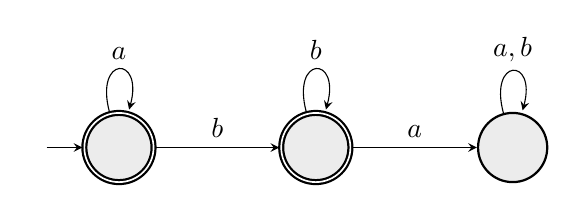
\begin{tikzpicture}
                            \node[state, accepting, initial] (q1) {};
                            \node[state, accepting, right of=q1] (q2) {};
                            \node[state, right of=q2] (q3) {};
                            \draw (q1) edge[loop above] node{$a$} (q1)
                            (q1) edge[above] node{$b$} (q2)
                            (q2) edge[loop above] node{$b$} (q2)
                            (q2) edge[above] node{$a$} (q3)
                            (q3) edge[loop above] node{$a,b$} (q3);
                        \end{tikzpicture}
                        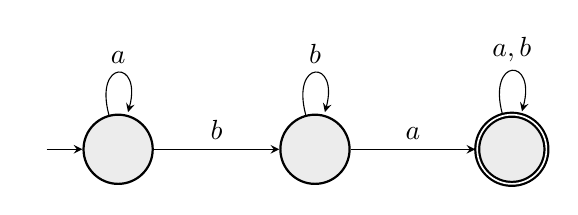
\begin{tikzpicture}
                            \node[state, initial] (q1) {};
                            \node[state, right of=q1] (q2) {};
                            \node[state, accepting, right of=q2] (q3) {};
                            \draw (q1) edge[loop above] node{$a$} (q1)
                            (q1) edge[above] node{$b$} (q2)
                            (q2) edge[loop above] node{$b$} (q2)
                            (q2) edge[above] node{$a$} (q3)
                            (q3) edge[loop above] node{$a,b$} (q3);
                        \end{tikzpicture}
                        \caption{$\overline{D}$ and $D$}
                    \end{figure}
              \item $E = \{w|w~\text{is any string not in }(ab^+)^{\ast}\}$

                    $\overline{E} = \{w|w~\text{is any string in }(ab^+)^{\ast}\}$

                    \begin{itemize}
                        \item assuming $ab^+$ means $a$ followed by one or more $b$.
                              \begin{figure}[H]
                                  \centering
                                  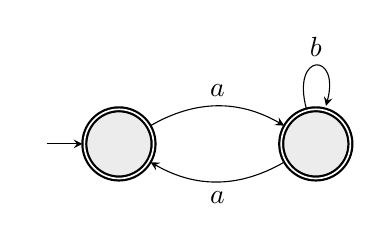
\begin{tikzpicture}
                                      \node[state, accepting, initial] (q1) {};
                                      \node[state, accepting, right of=q1] (q2) {};
                                      \draw (q1) edge[bend left, above] node{$a$} (q2)
                                      (q2) edge[bend left, below] node{$a$} (q1)
                                      (q2) edge[loop above] node{$b$} (q2);
                                  \end{tikzpicture}
                                  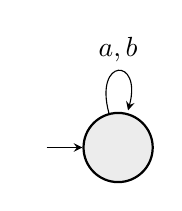
\begin{tikzpicture}
                                      \node[state, initial] (q1) {};
                                      \draw (q1) edge[loop above] node{$a,b$} (q1);
                                  \end{tikzpicture}
                                  \caption{$\overline{E}$ and $E$}
                              \end{figure}
                        \item assuming $ab^+$ means $ab$ one or more times.
                              \begin{figure}[H]
                                  \centering
                                  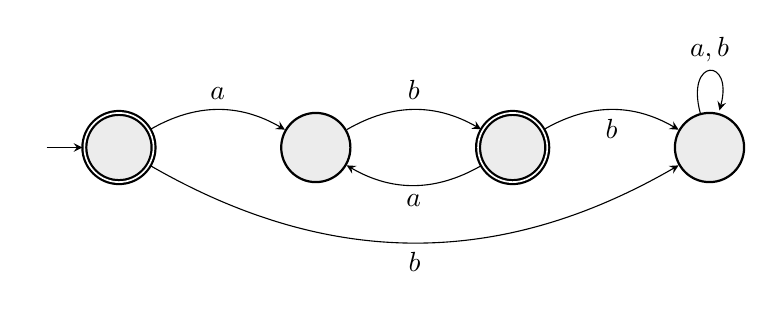
\begin{tikzpicture}
                                      \node[state, accepting, initial] (q1) {};
                                      \node[state, right of=q1] (q2) {};
                                      \node[state, accepting, right of=q2] (q3) {};
                                      \node[state, right of=q3] (q4) {};
                                      \draw (q1) edge[bend left, above] node{$a$} (q2)
                                      (q2) edge[bend left, above] node{$b$} (q3)
                                      (q3) edge[bend left, below] node{$a$} (q2)
                                      (q3) edge[bend left, below] node{$b$} (q4)
                                      (q1) edge[bend right, below] node{$b$} (q4)
                                      (q4) edge[loop above] node{$a,b$} (q4);
                                  \end{tikzpicture}
                                  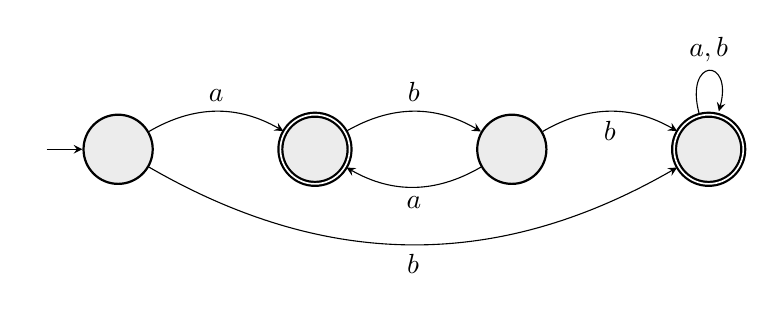
\begin{tikzpicture}
                                      \node[state, initial] (q1) {};
                                      \node[state, accepting, right of=q1] (q2) {};
                                      \node[state, right of=q2] (q3) {};
                                      \node[state, accepting, right of=q3] (q4) {};
                                      \draw (q1) edge[bend left, above] node{$a$} (q2)
                                      (q2) edge[bend left, above] node{$b$} (q3)
                                      (q3) edge[bend left, below] node{$a$} (q2)
                                      (q3) edge[bend left, below] node{$b$} (q4)
                                      (q1) edge[bend right, below] node{$b$} (q4)
                                      (q4) edge[loop above] node{$a,b$} (q4);
                                  \end{tikzpicture}
                                  \caption{$\overline{E}$ and $E$}
                              \end{figure}
                    \end{itemize}
              \item $F = \{w|w~\text{is any string not in }a^{\ast} \cup b^{\ast}\}$

                    $\overline{F} = \{w|w~\text{is any string in }a^{\ast} \cup b^{\ast}\}$
                    \begin{figure}[H]
                        \centering
                        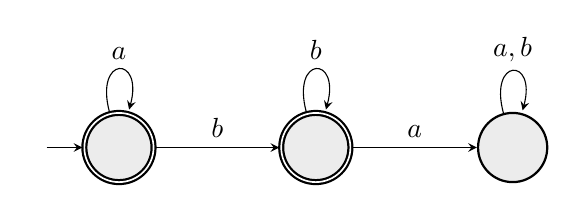
\begin{tikzpicture}
                            \node[state, accepting, initial] (q1) {};
                            \node[state, accepting, right of=q1] (q2) {};
                            \node[state, right of=q2] (q3) {};
                            \draw (q1) edge[loop above] node{$a$} (q1)
                            (q1) edge[above] node{$b$} (q2)
                            (q2) edge[loop above] node{$b$} (q2)
                            (q2) edge[above] node{$a$} (q3)
                            (q3) edge[loop above] node{$a,b$} (q3);
                        \end{tikzpicture}
                        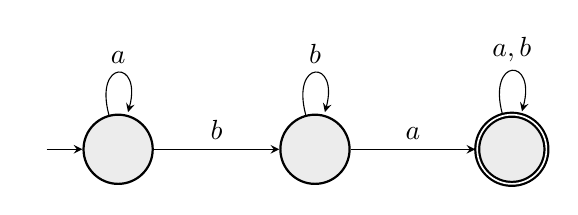
\begin{tikzpicture}
                            \node[state, initial] (q1) {};
                            \node[state, right of=q1] (q2) {};
                            \node[state, accepting, right of=q2] (q3) {};
                            \draw (q1) edge[loop above] node{$a$} (q1)
                            (q1) edge[above] node{$b$} (q2)
                            (q2) edge[loop above] node{$b$} (q2)
                            (q2) edge[above] node{$a$} (q3)
                            (q3) edge[loop above] node{$a,b$} (q3);
                        \end{tikzpicture}
                        \caption{$\overline{F}$ and $F$}
                    \end{figure}
              \item $G= \{w|w~\text{is any string that doesn’t contain exactly two }a\text{’s}\}$

                    $\overline{G} = \{w|w~\text{is any string that contains exactly two }a\text{’s}\}$
                    \begin{figure}[H]
                        \centering
                        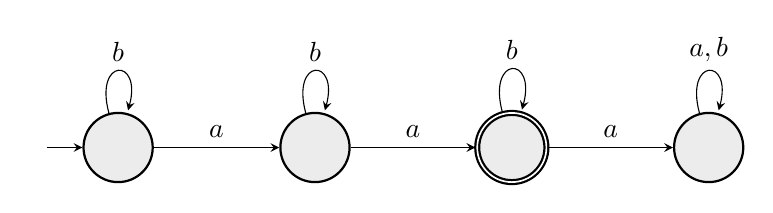
\begin{tikzpicture}
                            \node[state, initial] (q1) {};
                            \node[state, right of=q1] (q2) {};
                            \node[state, accepting, right of=q2] (q3) {};
                            \node[state, right of=q3] (q4) {};
                            \draw (q1) edge[loop above] node{$b$} (q1)
                            (q1) edge[above] node{$a$} (q2)
                            (q2) edge[loop above] node{$b$} (q2)
                            (q2) edge[above] node{$a$} (q3)
                            (q3) edge[loop above] node{$b$} (q3)
                            (q3) edge[above] node{$a$} (q4)
                            (q4) edge[loop above] node{$a,b$} (q4);
                        \end{tikzpicture}
                        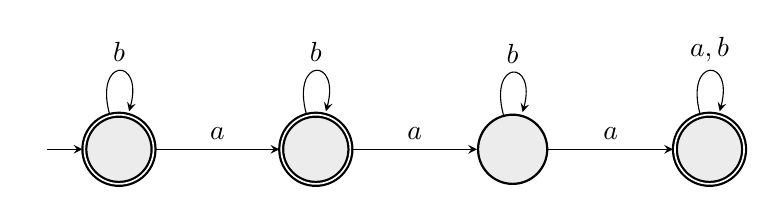
\begin{tikzpicture}
                            \node[state, accepting, initial] (q1) {};
                            \node[state, accepting, right of=q1] (q2) {};
                            \node[state, right of=q2] (q3) {};
                            \node[state, accepting, right of=q3] (q4) {};
                            \draw (q1) edge[loop above] node{$b$} (q1)
                            (q1) edge[above] node{$a$} (q2)
                            (q2) edge[loop above] node{$b$} (q2)
                            (q2) edge[above] node{$a$} (q3)
                            (q3) edge[loop above] node{$b$} (q3)
                            (q3) edge[above] node{$a$} (q4)
                            (q4) edge[loop above] node{$a,b$} (q4);
                        \end{tikzpicture}
                        \caption{$\overline{G}$ and $G$}
                    \end{figure}
              \item $H=\{w|w~\text{is any string except }a\text{ and }b\}$

                    $\overline{H} = \{w|w~\text{is string }a\text{ or }b\}$
                    \begin{figure}[H]
                        \centering
                        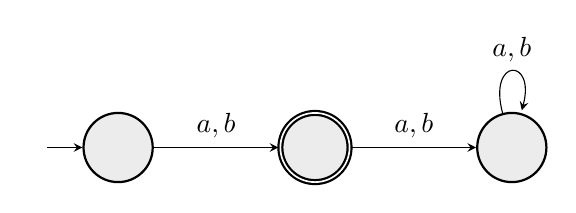
\begin{tikzpicture}
                            \node[state, initial] (q1) {};
                            \node[state, accepting, right of=q1] (q2) {};
                            \node[state, right of=q2] (q3) {};
                            \draw
                            (q1) edge[above] node{$a,b$} (q2)
                            (q2) edge[above] node{$a,b$} (q3)
                            (q3) edge[loop above] node{$a,b$} (q3);
                        \end{tikzpicture}
                        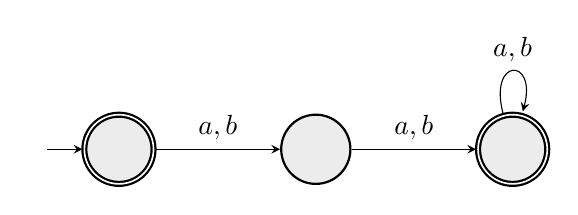
\begin{tikzpicture}
                            \node[state, accepting, initial] (q1) {};
                            \node[state, right of=q1] (q2) {};
                            \node[state, accepting, right of=q2] (q3) {};
                            \draw
                            (q1) edge[above] node{$a,b$} (q2)
                            (q2) edge[above] node{$a,b$} (q3)
                            (q3) edge[loop above] node{$a,b$} (q3);
                        \end{tikzpicture}
                        \caption{$\overline{H}$ and $H$}
                    \end{figure}
          \end{enumerate}

    \item[1.6]
          Give state diagrams of DFAs recognizing the following languages. In all parts,the alphabet is $\{0,1\}$.
          \begin{enumerate}
              \item $\{w|w~ \text{begins with a }1\text{ and ends with a }0\}$
                    \begin{figure}[H]
                        \centering
                        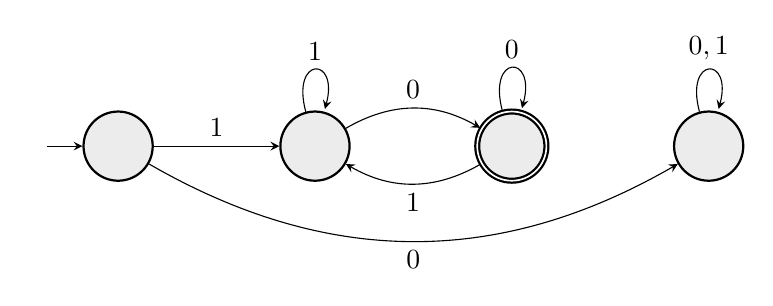
\begin{tikzpicture}
                            \node[state, initial] (q1) {};
                            \node[state, right of=q1] (q2) {};
                            \node[state, accepting, right of=q2] (q3) {};
                            \node[state, right of=q3] (q4) {};
                            \draw
                            (q1) edge[above] node{$1$} (q2)
                            (q2) edge[loop above] node{$1$} (q2)
                            (q2) edge[bend left, above] node{$0$} (q3)
                            (q3) edge[loop above] node{$0$} (q3)
                            (q3) edge[bend left, below] node{$1$} (q2)
                            (q1) edge[bend right, below] node{$0$} (q4)
                            (q4) edge[loop above] node{$0,1$} (q4);
                        \end{tikzpicture}
                    \end{figure}
              \item $\{w|w~ \text{contains at least three }1\text{'s}\}$
                    \begin{figure}[H]
                        \centering
                        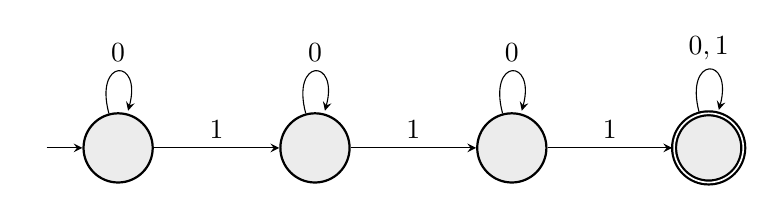
\begin{tikzpicture}
                            \node[state, initial] (q1) {};
                            \node[state, right of=q1] (q2) {};
                            \node[state, right of=q2] (q3) {};
                            \node[state, accepting, right of=q3] (q4) {};
                            \draw
                            (q1) edge[loop above] node{$0$} (q1)
                            (q1) edge[above] node{$1$} (q2)
                            (q2) edge[loop above] node{$0$} (q2)
                            (q2) edge[above] node{$1$} (q3)
                            (q3) edge[loop above] node{$0$} (q3)
                            (q3) edge[above] node{$1$} (q4)
                            (q4) edge[loop above] node{$0,1$} (q4);
                        \end{tikzpicture}
                    \end{figure}
              \item $\{w|w~ \text{contains the substring } 0101~ \text{(i.e., }w = x0101y\text{ for some }x\text{ and }y)\}$
                    \begin{figure}[H]
                        \centering
                        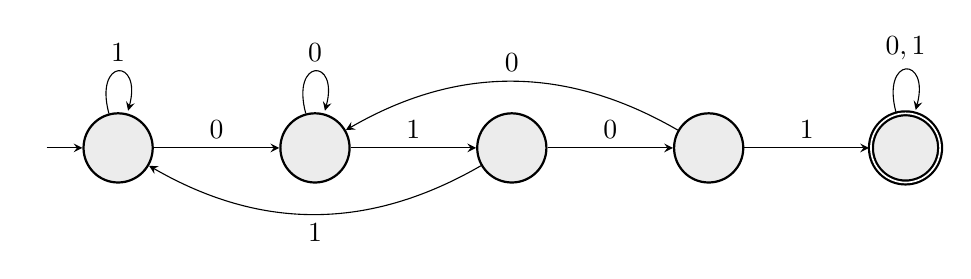
\begin{tikzpicture}
                            \node[state, initial] (q1) {};
                            \node[state, right of=q1] (q2) {};
                            \node[state, right of=q2] (q3) {};
                            \node[state, right of=q3] (q4) {};
                            \node[state, accepting, right of=q4] (q5) {};
                            \draw
                            (q1) edge[loop above] node{$1$} (q1)
                            (q1) edge[above] node{$0$} (q2)
                            (q2) edge[loop above] node{$0$} (q2)
                            (q2) edge[above] node{$1$} (q3)
                            (q3) edge[above] node{$0$} (q4)
                            (q4) edge[above] node{$1$} (q5)
                            (q5) edge[loop above] node{$0,1$} (q5)
                            (q3) edge[bend left, below] node{$1$} (q1)
                            (q4) edge[bend right, above] node{$0$} (q2);
                        \end{tikzpicture}
                    \end{figure}
              \item $\{w|w~ \text{has length at least }3\text{ and its third symbol is a }0\}$
                    \begin{figure}[H]
                        \centering
                        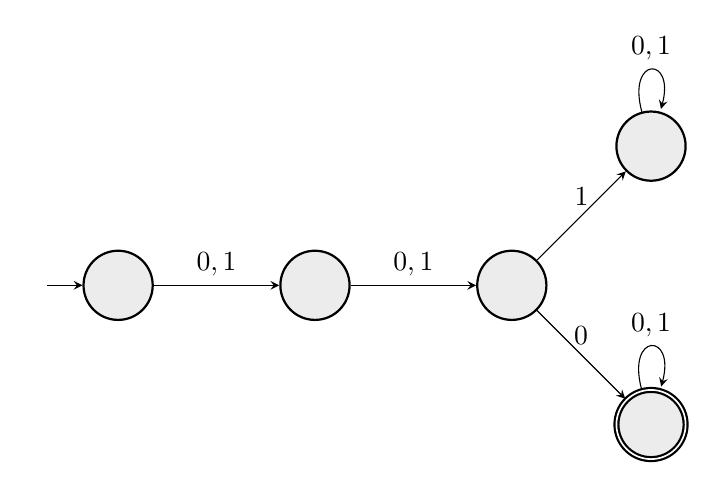
\begin{tikzpicture}
                            \node[state, initial] (q1) {};
                            \node[state, right of=q1] (q2) {};
                            \node[state, right of=q2] (q3) {};
                            \node[state, accepting, below right of=q3] (q4) {};
                            \node[state, above right of=q3] (q5) {};
                            \draw
                            (q1) edge[above] node{$0,1$} (q2)
                            (q2) edge[above] node{$0,1$} (q3)
                            (q3) edge[above] node{$0$} (q4)
                            (q3) edge[above] node{$1$} (q5)
                            (q4) edge[loop above] node{$0,1$} (q4)
                            (q5) edge[loop above] node{$0,1$} (q5);
                        \end{tikzpicture}
                    \end{figure}

              \item $\{w|w~ \text{starts with }0\text{ and has odd length, or starts with }1\text{ and has even length}\}$
                    \begin{figure}[H]
                        \centering
                        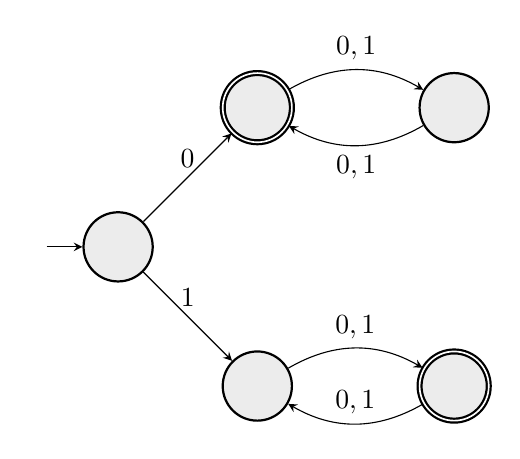
\begin{tikzpicture}
                            \node[state, initial] (q1) {};
                            \node[state, accepting, above right of=q1] (q2) {};
                            \node[state, below right of=q1] (q3) {};
                            \node[state, right of=q2] (q4) {};
                            \node[state, accepting, right of=q3] (q5) {};
                            \draw
                            (q1) edge[above] node{$0$} (q2)
                            (q1) edge[above] node{$1$} (q3)
                            (q2) edge[bend left, above] node{$0,1$} (q4)
                            (q4) edge[bend left, below] node{$0,1$} (q2)
                            (q3) edge[bend left, above] node{$0,1$} (q5)
                            (q5) edge[bend left, above] node{$0,1$} (q3);
                        \end{tikzpicture}
                    \end{figure}
              \item $\{w|w~ \text{doesn't contain the substring }110\}$
                    \begin{figure}[H]
                        \centering
                        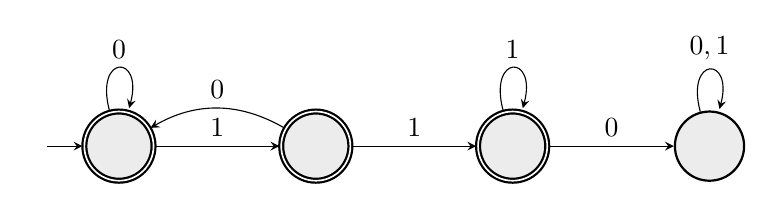
\begin{tikzpicture}
                            \node[state, accepting, initial] (q1) {};
                            \node[state, accepting, right of=q1] (q2) {};
                            \node[state, accepting, right of=q2] (q3) {};
                            \node[state, right of=q3] (q4) {};
                            \draw
                            (q1) edge[above] node{$1$} (q2)
                            (q1) edge[loop above] node{$0$} (q1)
                            (q2) edge[above] node{$1$} (q3)
                            (q2) edge[bend right, above] node{$0$} (q1)
                            (q3) edge[above] node{$0$} (q4)
                            (q3) edge[loop above] node{$1$} (q3)
                            (q4) edge[loop above] node{$0,1$} (q4);
                        \end{tikzpicture}
                    \end{figure}
              \item $\{w|\text{the length of }w\text{ is at most }5\}$

                    \begin{figure}[H]
                        \centering
                        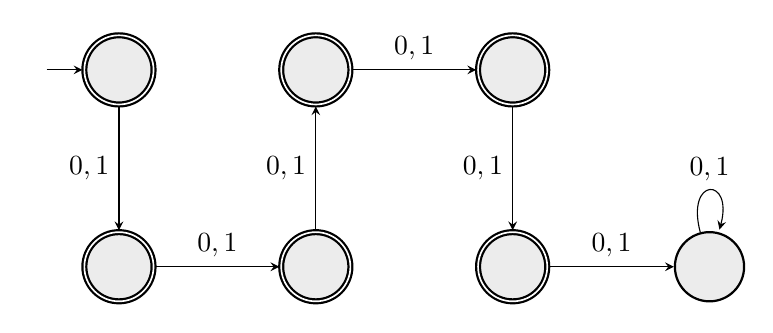
\begin{tikzpicture}
                            \node[state, accepting, initial] (q1) {};
                            \node[state, accepting, below of=q1] (q2) {};
                            \node[state, accepting, right of=q2] (q3) {};
                            \node[state, accepting, above of=q3] (q4) {};
                            \node[state, accepting, right of=q4] (q5) {};
                            \node[state, accepting, below of=q5] (q6) {};
                            \node[state, right of=q6] (q7) {};
                            \draw
                            (q7) edge[loop above] node{$0,1$} (q7)
                            (q1) edge[left] node{$0,1$} (q2)
                            (q2) edge[above] node{$0,1$} (q3)
                            (q3) edge[left] node{$0,1$} (q4)
                            (q4) edge[above] node{$0,1$} (q5)
                            (q5) edge[left] node{$0,1$} (q6)
                            (q6) edge[above] node{$0,1$} (q7);
                        \end{tikzpicture}
                    \end{figure}

              \item $\{w|w~ \text{is any string except }11\text{ and }111\}$
                    \begin{figure}[H]
                        \centering
                        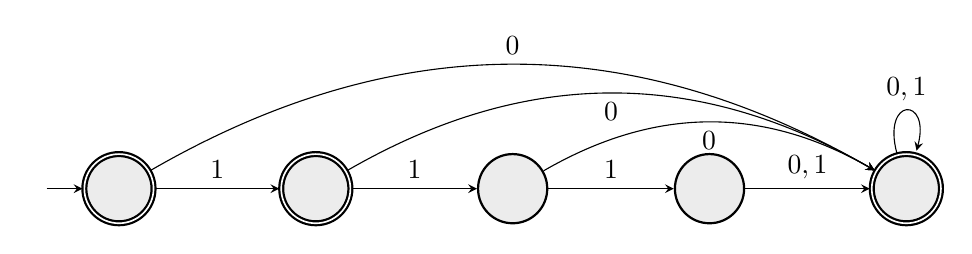
\begin{tikzpicture}
                            \node[state, accepting, initial] (q1) {};
                            \node[state, accepting, right of=q1] (q2) {};
                            \node[state, right of=q2] (q3) {};
                            \node[state, right of=q3] (q4) {};
                            \node[state, accepting, right of=q4] (q5) {};
                            \draw
                            (q1) edge[above] node{$1$} (q2)
                            (q1) edge[bend left, above] node{$0$} (q5)
                            (q2) edge[above] node{$1$} (q3)
                            (q2) edge[bend left, below ] node{$0$} (q5)
                            (q3) edge[above] node{$1$} (q4)
                            (q3) edge[bend left, below] node{$0$} (q5)
                            (q4) edge[above] node{$0,1$} (q5)
                            (q5) edge[loop above] node{$0,1$} (q5);
                        \end{tikzpicture}
                    \end{figure}
              \item $\{w|\text{ every odd position of }w\text{ is a }1\}$
                    \begin{figure}[H]
                        \centering
                        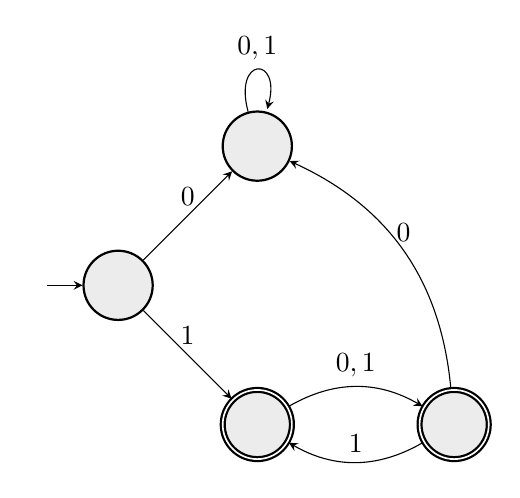
\begin{tikzpicture}
                            \node[state, initial] (q1) {};
                            \node[state, above right of=q1] (q2) {};
                            \node[state, accepting, below right of=q1] (q3) {};
                            \node[state, accepting, right of=q3] (q5) {};
                            \draw
                            (q1) edge[above] node{$0$} (q2)
                            (q1) edge[above] node{$1$} (q3)
                            (q2) edge[loop above] node{$0,1$} (q2)
                            (q3) edge[bend left, above] node{$0,1$} (q5)
                            (q5) edge[bend left, above] node{$1$} (q3)
                            (q5) edge[bend right, above] node{$0$} (q2);
                        \end{tikzpicture}
                    \end{figure}
              \item $\{w|w~ \text{contains at least two }0\text{'s and at most one }1\}$
                    \begin{figure}[H]
                        \centering
                        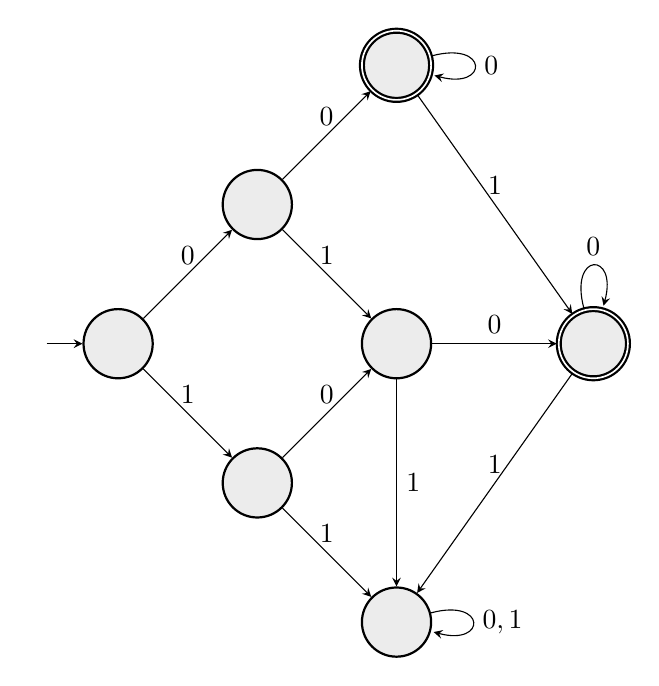
\begin{tikzpicture}
                            \node[state, initial] (q1) {};
                            \node[state, above right of=q1] (q2) {};
                            \node[state, below right of=q1] (q3) {};
                            \node[state, below right of=q2] (q4) {};
                            \node[state, accepting, above right of=q2] (q5) {};
                            \node[state, below right of=q3] (q8) {};
                            \node[state, accepting, right of=q4] (q6) {};
                            \draw
                            (q1) edge[above] node{$0$} (q2)
                            (q1) edge[above] node{$1$} (q3)
                            (q2) edge[above] node{$0$} (q5)
                            (q2) edge[above] node{$1$} (q4)
                            (q3) edge[above] node{$0$} (q4)
                            (q3) edge[above] node{$1$} (q8)
                            (q4) edge[above] node{$0$} (q6)
                            (q4) edge[right] node{$1$} (q8)
                            (q5) edge[above] node{$1$} (q6)
                            (q5) edge[loop right] node{$0$} (q5)
                            (q6) edge[loop above] node{$0$} (q6)
                            (q8) edge[loop right] node{$0,1$} (q8)
                            (q6) edge[above] node{$1$} (q8);
                        \end{tikzpicture}
                    \end{figure}
              \item $\{\epsilon,0\}$
                    \begin{figure}[H]
                        \centering
                        \begin{tikzpicture}
                            \node[state, initial, accepting] (q1) {};
                            \node[state, accepting, above right of=q1] (q2) {};
                            \node[state, below right of=q1] (q3) {};
                            \draw
                            (q1) edge[above] node{$0$} (q2)
                            (q1) edge[right] node{$1$} (q3)
                            (q2) edge[right] node{$0,1$} (q3)
                            (q3) edge[loop right] node{$0,1$} (q3);
                        \end{tikzpicture}
                    \end{figure}
              \item $\{w|w~ \text{contains an even number of }0\text{'s, or contains exactly two }1\text{'s}\}$
                    \begin{figure}[H]
                        \centering
                        \begin{tikzpicture}
                            \node[state, initial, accepting] (q1) {};
                            \node[state, accepting, above right of=q1] (q2) {};
                            \node[state, below right of=q1] (q3) {};
                            \node[state, accepting, right of=q3] (q4) {};
                            \node[state, right of=q2] (q5) {};
                            \node[state, accepting, above right of=q2] (q6) {};
                            \node[state, accepting, right of=q6] (q7) {};
                            \node[state, accepting, above right of=q6] (q8) {};
                            \node[state, right of=q8] (q9) {};
                            \draw
                            (q1) edge[above] node{$1$} (q2)
                            (q1) edge[right] node{$0$} (q3)
                            (q3) edge[below] node{$1$} (q5)
                            (q4) edge[bend right, below] node{$1$} (q2)
                            (q3) edge[bend right, above] node{$0$} (q4)
                            (q4) edge[bend right, below] node{$0$} (q3)
                            (q2) edge[bend right, above] node{$0$} (q5)
                            (q2) edge[right, above] node{$1$} (q6)
                            (q5) edge[right, below] node{$1$} (q7)
                            (q5) edge[bend right, below] node{$0$} (q2)
                            (q6) edge[bend right, above] node{$0$} (q7)
                            (q7) edge[bend right, below] node{$0$} (q6)
                            (q6) edge[right, above] node{$1$} (q8)
                            (q7) edge[right, below] node{$1$} (q9)
                            (q8) edge[bend right, above] node{$0$} (q9)
                            (q9) edge[bend right, below] node{$0$} (q8);
                        \end{tikzpicture}
                    \end{figure}
              \item The empty set
                    \begin{figure}[H]
                        \centering
                        \begin{tikzpicture}
                            \node[state, initial] (q1) {};
                            \draw
                            (q1) edge[loop right] node{$0,1$} (q1);
                        \end{tikzpicture}
                    \end{figure}
              \item All strings except the empty string
                    \begin{figure}[H]
                        \centering
                        \begin{tikzpicture}
                            \node[state, initial] (q1) {};
                            \node[state, accepting, right of=q1] (q2) {};
                            \draw
                            (q1) edge[above] node{$0,1$} (q2)
                            (q2) edge[loop above] node{$0,1$} (q2);
                        \end{tikzpicture}
                    \end{figure}
          \end{enumerate}
\end{enumerate}

\begin{enumerate}
    \item[1.7]
          Give state diagrams of NFAs with the specified number of states recognizing each of the following languages. In all parts, the alphabet is {0,1}.
          \begin{enumerate}
              \item The language $\{w|w~ \text{ends with }00\}$ with three states
                    \begin{figure}[H]
                        \centering
                        \begin{tikzpicture}
                            \node[state, initial] (q1) {};
                            \node[state, right of=q1] (q2) {};
                            \node[state, accepting, right of=q2] (q3) {};
                            \draw
                            (q1) edge[above] node{$0$} (q2)
                            (q2) edge[above] node{$0$} (q3)
                            (q1) edge[loop above] node{$0,1$} (q1);
                        \end{tikzpicture}
                    \end{figure}
              \item The language of Exercise 1.6c with five states
                    \begin{figure}[H]
                        \centering
                        \begin{tikzpicture}
                            \node[state, initial] (q1) {};
                            \node[state, right of=q1] (q2) {};
                            \node[state, right of=q2] (q3) {};
                            \node[state, right of=q3] (q4) {};
                            \node[state, accepting, right of=q4] (q5) {};
                            \draw
                            (q1) edge[loop above] node{$1$} (q1)
                            (q1) edge[above] node{$0$} (q2)
                            (q2) edge[loop above] node{$0$} (q2)
                            (q2) edge[above] node{$1$} (q3)
                            (q3) edge[above] node{$0$} (q4)
                            (q4) edge[above] node{$1$} (q5)
                            (q5) edge[loop above] node{$0,1$} (q5)
                            (q3) edge[bend left, below] node{$1$} (q1)
                            (q4) edge[bend right, above] node{$0$} (q2);
                        \end{tikzpicture}
                    \end{figure}
              \item The language of Exercise 1.6l with six states
                    \begin{figure}[H]
                        \centering
                        \begin{tikzpicture}
                            \node[state, accepting, initial] (q1) {};
                            \node[state, above right of=q1] (q2) {};
                            \node[state, accepting, below right of=q1] (q3) {};
                            \node[state, right of=q3] (q4) {};
                            \node[state, right of=q2] (q5) {};
                            \node[state, accepting, right of=q5] (q6) {};
                            \draw
                            (q1) edge[right] node{$\epsilon$} (q2)
                            (q1) edge[above] node{$1$} (q3)
                            (q3) edge[above] node{$1$} (q4)
                            (q1) edge[loop above] node{$0$} (q1)
                            (q3) edge[loop above] node{$0$} (q3)
                            (q4) edge[loop above] node{$0$} (q4)
                            (q2) edge[loop above] node{$0,1$} (q2)
                            (q5) edge[loop above] node{$1$} (q5)
                            (q6) edge[loop above] node{$0,1$} (q6)
                            (q2) edge[right, below] node{$0$} (q5)
                            (q5) edge[right, below] node{$0$} (q6);
                        \end{tikzpicture}
                    \end{figure}
              \item The language $\{0\}$ with two states
                    \begin{figure}[H]
                        \centering
                        \begin{tikzpicture}
                            \node[state, initial] (q1) {};
                            \node[state, accepting, right of=q1] (q2) {};
                            \draw
                            (q1) edge[above] node{$0$} (q2);
                        \end{tikzpicture}
                    \end{figure}
              \item The language $0^\ast1^\ast0+$ with three states
                    \begin{figure}[H]
                        \centering
                        \begin{tikzpicture}
                            \node[state, initial] (q1) {};
                            \node[state, right of=q1] (q2) {};
                            \node[state, accepting, right of=q2] (q3) {};
                            \draw
                            (q1) edge[above] node{$\epsilon$} (q2)
                            (q2) edge[above] node{$0$} (q3)
                            (q1) edge[loop above] node{$0$} (q1)
                            (q2) edge[loop above] node{$1$} (q2)
                            (q3) edge[loop above] node{$0$} (q3);
                        \end{tikzpicture}
                    \end{figure}
              \item The language $1^\ast(001+)^\ast$ with three states
                    \begin{figure}[H]
                        \centering
                        \begin{tikzpicture}
                            \node[state, accepting, initial] (q1) {};
                            \node[state, right of=q1] (q2) {};
                            \node[state, below right of=q1] (q3) {};
                            \draw
                            (q1) edge[above] node{$0$} (q2)
                            (q2) edge[right] node{$0$} (q3)
                            (q3) edge[left] node{$1$} (q1)
                            (q1) edge[loop above] node{$1$} (q1);
                        \end{tikzpicture}
                    \end{figure}
              \item The language ${\epsilon}$ with one state
                    \begin{figure}[H]
                        \centering
                        \begin{tikzpicture}
                            \node[state, initial, accepting] (q1) {};
                        \end{tikzpicture}
                    \end{figure}
              \item The language $0^\ast$ with one state
                    \begin{figure}[H]
                        \centering
                        \begin{tikzpicture}
                            \node[state, initial, accepting] (q1) {};
                            \draw
                            (q1) edge[loop above] node{$0$} (q1);
                        \end{tikzpicture}
                    \end{figure}
          \end{enumerate}
    \item[1.8]
          Use the construction in the proof of Theorem 1.45 to give the state diagrams of NFAs recognizing the union of the languages described in:
          \begin{enumerate}
              \item  Exercises 1.6a and 1.6b
                    \begin{figure}[H]
                        \centering
                        \begin{tikzpicture}
                            \node[state, initial] (q0) {};
                            \node[state, above right of=q0] (q1) {};
                            \node[state, right of=q1] (q2) {};
                            \node[state, accepting, right of=q2] (q3) {};
                            \node[state, right of=q3] (q4) {};
                            \node[state, below right of=q0] (bq1) {};
                            \node[state, right of=bq1] (bq2) {};
                            \node[state, right of=bq2] (bq3) {};
                            \node[state, accepting, right of=bq3] (bq4) {};
                            \draw
                            (q0) edge[above, blue] node{$\epsilon$} (q1)
                            (q0) edge[above, blue] node{$\epsilon$} (bq1)
                            (q1) edge[above] node{$1$} (q2)
                            (q2) edge[loop above] node{$1$} (q2)
                            (q2) edge[bend left, above] node{$0$} (q3)
                            (q3) edge[loop above] node{$0$} (q3)
                            (q3) edge[bend left, below] node{$1$} (q2)
                            (q1) edge[bend right, below] node{$0$} (q4)
                            (q4) edge[loop above] node{$0,1$} (q4)
                            (q1) edge[loop above] node{$0$} (q1)
                            (bq1) edge[above] node{$1$} (bq2)
                            (bq2) edge[loop above] node{$0$} (bq2)
                            (bq2) edge[above] node{$1$} (bq3)
                            (bq3) edge[loop above] node{$0$} (bq3)
                            (bq3) edge[above] node{$1$} (bq4)
                            (bq4) edge[loop above] node{$0,1$} (bq4);
                        \end{tikzpicture}
                    \end{figure}
              \item Exercises 1.6c and 1.6f
                    \begin{figure}[H]
                        \centering
                        \begin{tikzpicture}
                            \node[state, initial] (q0) {};
                            \node[state, above right of=q0] (q1) {};
                            \node[state, right of=q1] (q2) {};
                            \node[state, right of=q2] (q3) {};
                            \node[state, right of=q3] (q4) {};
                            \node[state, accepting, right of=q4] (q5) {};
                            \node[state, accepting, below right of=q0] (bq1) {};
                            \node[state, accepting, right of=bq1] (bq2) {};
                            \node[state, accepting, right of=bq2] (bq3) {};
                            \node[state, right of=bq3] (bq4) {};
                            \draw
                            (q0) edge[above, blue] node{$\epsilon$} (q1)
                            (q0) edge[above, blue] node{$\epsilon$} (bq1)
                            (q1) edge[loop above] node{$1$} (q1)
                            (q1) edge[above] node{$0$} (q2)
                            (q2) edge[loop above] node{$0$} (q2)
                            (q2) edge[above] node{$1$} (q3)
                            (q3) edge[above] node{$0$} (q4)
                            (q4) edge[above] node{$1$} (q5)
                            (q5) edge[loop above] node{$0,1$} (q5)
                            (q3) edge[bend left, below] node{$1$} (q1)
                            (q4) edge[bend right, above] node{$0$} (q2)
                            (bq1) edge[above] node{$1$} (bq2)
                            (bq1) edge[loop above] node{$0$} (bq1)
                            (bq2) edge[above] node{$1$} (bq3)
                            (bq2) edge[bend right, above] node{$0$} (bq1)
                            (bq3) edge[above] node{$0$} (bq4)
                            (bq3) edge[loop above] node{$1$} (bq3)
                            (bq4) edge[loop above] node{$0,1$} (bq4);
                        \end{tikzpicture}
                    \end{figure}
          \end{enumerate}
    \item[1.9]
          Use the construction in the proof of Theorem 1.47 to give the state diagrams of NFAs recognizing the concatenation of the languages described in
          \begin{enumerate}
              \item Exercises 1.6g and 1.6i.
                    \begin{figure}[H]
                        \centering
                        \begin{tikzpicture}
                            \node[state, accepting, initial] (q1) {};
                            \node[state, accepting, below of=q1] (q2) {};
                            \node[state, accepting, right of=q2] (q3) {};
                            \node[state, accepting, above of=q3] (q4) {};
                            \node[state, accepting, right of=q4] (q5) {};
                            \node[state, accepting, below of=q5] (q6) {};
                            \node[state, right of=q6] (q7) {};
                            \node[state, below of=q7] (bq1) {};
                            \node[state, above right of=bq1] (bq2) {};
                            \node[state, accepting, below right of=bq1] (bq3) {};
                            \node[state, accepting, right of=bq3] (bq5) {};
                            \draw
                            (q7) edge[loop above] node{$0,1$} (q7)
                            (q1) edge[left] node{$0,1$} (q2)
                            (q2) edge[above] node{$0,1$} (q3)
                            (q3) edge[left] node{$0,1$} (q4)
                            (q4) edge[above] node{$0,1$} (q5)
                            (q5) edge[left] node{$0,1$} (q6)
                            (q6) edge[above] node{$0,1$} (q7)
                            
                            (bq1) edge[above] node{$0$} (bq2)
                            (bq1) edge[above] node{$1$} (bq3)
                            (bq2) edge[loop above] node{$0,1$} (bq2)
                            (bq3) edge[bend left, above] node{$0,1$} (bq5)
                            (bq5) edge[bend left, above] node{$1$} (bq3)
                            (bq5) edge[bend right, above] node{$0$} (bq2)
                            
                            (q1) edge[left, below, blue] node{$\epsilon$} (bq1)
                            (q2) edge[left, below, blue] node{$\epsilon$} (bq1)
                            (q3) edge[left, below, blue] node{$\epsilon$} (bq1)
                            (q4) edge[left, below, blue] node{$\epsilon$} (bq1)
                            (q5) edge[left, below, blue] node{$\epsilon$} (bq1);
                        \end{tikzpicture}
                    \end{figure}
              \item Exercises 1.6b and 1.6m.
                    \begin{figure}[H]
                        \centering
                        \begin{tikzpicture}
                            \node[state, initial] (q1) {};
                            \node[state, right of=q1] (q2) {};
                            \node[state, right of=q2] (q3) {};
                            \node[state, accepting, right of=q3] (q4) {};
                            \node[state, right of=q4] (bq1) {};
                            \draw
                            (q1) edge[loop above] node{$0$} (q1)
                            (q1) edge[above] node{$1$} (q2)
                            (q2) edge[loop above] node{$0$} (q2)
                            (q2) edge[above] node{$1$} (q3)
                            (q3) edge[loop above] node{$0$} (q3)
                            (q3) edge[above] node{$1$} (q4)
                            (q4) edge[loop above] node{$0,1$} (q4)
                            (q4) edge[above, blue] node{$\epsilon$} (bq1)
                            (bq1) edge[loop right] node{$0,1$} (bq1);
                        \end{tikzpicture}
                    \end{figure}
          \end{enumerate}
          
    \item [1.10]
          Use the construction in the proof of Theorem 1.49 to give the state diagrams of NFAs recognizing the star of the languages described in 
          \begin{enumerate}
              \item Exercise 1.6b.
                    \begin{figure}[H]
                        \centering
                        \begin{tikzpicture}
                            \node[state, accepting, initial] (q0) {};
                            \node[state, right of=q0] (q1) {};
                            \node[state, right of=q1] (q2) {};
                            \node[state, right of=q2] (q3) {};
                            \node[state, accepting, right of=q3] (q4) {};
                            \draw
                            (q0) edge[above] node{$\epsilon$} (q1)
                            
                            (q1) edge[loop above] node{$0$} (q1)
                            (q1) edge[above] node{$1$} (q2)
                            (q2) edge[loop above] node{$0$} (q2)
                            (q2) edge[above] node{$1$} (q3)
                            (q3) edge[loop above] node{$0$} (q3)
                            (q3) edge[above] node{$1$} (q4)
                            (q4) edge[loop above] node{$0,1$} (q4)
                            
                            (q4) edge[bend left, below] node{$\epsilon$} (q1);
                        \end{tikzpicture}
                    \end{figure}
              \item Exercise 1.6j.
                    \begin{figure}[H]
                        \centering
                        \begin{tikzpicture}
                            \node[state, initial] (q0) {};
                            \node[state, right of=q0] (q1) {};
                            \node[state, above right of=q1] (q2) {};
                            \node[state, below right of=q1] (q3) {};
                            \node[state, below right of=q2] (q4) {};
                            \node[state, accepting, above right of=q2] (q5) {};
                            \node[state, below right of=q3] (q8) {};
                            \node[state, accepting, right of=q4] (q6) {};
                            \draw
                            (q0) edge[above] node{$\epsilon$} (q1)
                            (q1) edge[above] node{$0$} (q2)
                            (q1) edge[above] node{$1$} (q3)
                            (q2) edge[above] node{$0$} (q5)
                            (q2) edge[above] node{$1$} (q4)
                            (q3) edge[above] node{$0$} (q4)
                            (q3) edge[above] node{$1$} (q8)
                            (q4) edge[above] node{$0$} (q6)
                            (q4) edge[right] node{$1$} (q8)
                            (q5) edge[above] node{$1$} (q6)
                            (q5) edge[loop right] node{$0$} (q5)
                            (q6) edge[loop above] node{$0$} (q6)
                            (q8) edge[loop right] node{$0,1$} (q8)
                            (q6) edge[above] node{$1$} (q8)
                            
                            (q5) edge[bend left, below] node{$\epsilon$} (q1)
                            (q6) edge[bend left, below] node{$\epsilon$} (q1);
                        \end{tikzpicture}
                    \end{figure}
              \item Exercise 1.6m.
                    \begin{figure}[H]
                        \centering
                        \begin{tikzpicture}
                            \node[state, initial, accepting] (q0) {};
                            \node[state, right of=q0] (q1) {};
                            \draw
                            (q0) edge[above] node{$\epsilon$} (q1)
                            (q1) edge[loop right] node{$0,1$} (q1);
                        \end{tikzpicture}
                    \end{figure}
          \end{enumerate}
          
    \item [1.11]
          Prove that every NFA can be converted to an equivalent one that has a single accept state.
          
          It is enough to show that every NFA can be converted to an equivalent one that has a single accept state and no transitions into the accept state. Let $N = (Q, \Sigma, \delta, q_0, F)$ be an NFA. We construct an NFA $N' = (Q \cup \{q_f\}, \Sigma, \delta', q_0, \{q_f\})$ where $\delta'$ is the same as $\delta$ with additional transitions: for each $q \in F$ $\delta'(q, \epsilon) = \{q_f\}$. It is clear that $L(N) = L(N')$ and that $N'$ has a single accept state. Therefore, every NFA can be converted to an equivalent one that has a single accept state.
          
    \item [1.12]
          
          Let \[D = \{w|w~ \text{contains an even number of }a\text{’s and an odd number of }b\text{’s}\]
          \[ \text{and does not contain the substring }ab\}\] Give a DFA with five states that recognizes $D$ and a regular expression that generates $D$. (Suggestion: Describe $D$ more simply.)
          
          $$D = \{w|w~ \text{contains odd number of }b\text{'s followed by even number of }a\text{'s} \}$$
          
          \begin{figure}[H]
              \centering
              \begin{tikzpicture}
                  \node[state, initial] (q0) {};
                  \node[state, accepting, right of=q0] (q1) {};
                  \node[state, right of=q1] (q2) {};
                  \node[state, right of=q2] (q3) {};
                  \node[state, above of=q1] (q5) {};
                  \draw
                  (q0) edge[above] node{$b$} (q1)
                  (q0) edge[bend right, below] node{$a$} (q2)
                  (q1) edge[bend left, left] node{$b$} (q5)
                  (q5) edge[bend left, left] node{$b$} (q1)
                  (q1) edge[bend left, below] node{$a$} (q2)
                  (q2) edge[bend left, above] node{$a$} (q1)
                  (q2) edge[below] node{$b$} (q3)
                  (q5) edge[below] node{$a$} (q3)
                  (q3) edge[loop above] node{$a,b$} (q3);
              \end{tikzpicture}
          \end{figure}
          
          The regular expression that generates $D$ is $b(bb)^{\ast}(aa)^{\ast}$.
\end{enumerate}

\begin{enumerate}

    \item [1.13]
          
          Let $F$ be the language of all strings over $\{0,1\}$ that do not contain a pair of $1$s that are separated by an odd number of symbols. Give the state diagram of a DFA with five states that recognizes $F$. (You may find it helpful first to find a 4-state NFA for the complement of $F$.) blab
          
          $\overline{F} = \{w|w~ \text{contains a pair of }1\text{'s that are separated by an odd number of symbols}\}$
          
          \begin{figure}[H]
              \centering
              \begin{tikzpicture}
                  \node[state, initial] (q0) {};
                  \node[state, right of=q0] (q1) {};
                  \node[state, above of=q1] (q2) {};
                  \node[state, accepting, right of=q1] (q3) {};
                  \draw
                  (q0) edge[above] node{$1$} (q1)
                  (q0) edge[bend right, below] node{$1$} (q2)
                  (q2) edge[above] node{$1$} (q3)
                  (q2) edge[bend right, above] node{$1$} (q3)
                  (q3) edge[loop above] node{$0$} (q3);
              \end{tikzpicture}
              \caption{NFA with four states that recognizes $\overline{F}$}
          \end{figure}
    \item [1.14]
          \begin{enumerate}
              \item Show that if $M$ is a DFA that recognizes language $B$, swapping the accept and nonaccept states in $M$ yields a new DFA recognizing the complement of $B$.Conclude that the class of regular languages is closed under complement.
                    
                    Every state in DFA has a transition for every symbol in the alphabet. For every possible word, the DFA will end up in either an accept state or a nonaccept state. If we swap the accept and nonaccept states in $M$, the new DFA will accept the complement of the language $B$.
                    
              \item Show by giving an example that if $M$ is an NFA that recognizes language $C$, swapping the accept and non-accept states in $M$ doesn’t necessarily yield a new NFA that recognizes the complement of $C$. Is the class of languages recognized by NFAs closed under complement? Explain your answer.
                    
                    \begin{figure}[H]
                        \centering
                        \begin{tikzpicture}
                            \node[state, initial] (q0) {};
                            \node[state, accepting, right of=q0] (q1) {};
                            \draw
                            (q0) edge[above] node{$0,1$} (q1)
                            (q0) edge[loop above] node{$0$} (q0);
                        \end{tikzpicture}
                        \caption{example NFA}
                        \begin{tikzpicture}
                            \node[state, accepting, initial] (q0) {};
                            \node[state, right of=q0] (q1) {};
                            \draw
                            (q0) edge[above] node{$0,1$} (q1)
                            (q0) edge[loop above] node{$0$} (q0);
                        \end{tikzpicture}
                        \caption{example NFA with changed states acceptance}
                    \end{figure}
                    
                    NFA accepts a string if there is at least one path that leads to an accept state. If we swap the accept and non-accept states in $M$, the new NFA will not necessarily accept the complement of the language $C$. The class of languages recognized by NFAs is not closed under complement.
          \end{enumerate}
    \item [1.15]
          Give a counter example to show that the following construction fails to prove Theorem 1.49, the closure of the class of regular languages under the star operation. Let $N_1 = (Q_1,\Sigma,\delta_1,q_1,F_1)$ recognize $A_1$. Construct $N = (Q_1,\Sigma,\delta,q_1,F)$ as follows. $N$ is supposed to recognize $A_1^\ast$.
          \begin{enumerate}
              \item The states of $N$ are the states of $N_1$.
              \item The start state of $N$ is the same as the start state of $N_1$.
              \item $F =\{q_1\} \cup F_1$.
                    
                    The accept states F are the old accept states plus its start state.
              \item Define $\delta$ so that for any $q \in Q_1$ and any $a \in \Sigma_\epsilon$,
                    $$\delta(q,a)=
                        \begin{cases}
                            \delta_1(q,a)              & q \notin F_1~ \text{or }a \neq \epsilon \\
                            \delta_1(q,a) \cup \{q_1\} & q \in F_1~ \text{and }a = \epsilon.
                        \end{cases}
                    $$
          \end{enumerate}
          (Suggestion: Show this construction graphically, as in Figure 1.50.)
          
          \begin{figure}[H]
              \centering
              \begin{tikzpicture}

                  \node[state, initial] (q0) {};
                  \node[state, right of=q0, minimum size=0.5cm] (q02) {};
                  \node[state, above of=q02, minimum size=0.5cm] (q01) {};
                  \node[state, below of=q02, minimum size=0.5cm] (q03) {};
                  \node[state, accepting, above right of=q02] (q2) {};
                  \node[state, accepting, below of=q2] (q3) {};
              \end{tikzpicture}
              \caption{NFA $N_1$}
          \end{figure}
          \begin{figure}[H]
              \centering
              \begin{tikzpicture}
                  \node[state, accepting, initial] (q0) {};
                  \node[state, right of=q0, minimum size=0.5cm] (q02) {};
                  \node[state, above of=q02, minimum size=0.5cm] (q01) {};
                  \node[state, below of=q02, minimum size=0.5cm] (q03) {};
                  \node[state, accepting, above right of=q02] (q2) {};
                  \node[state, accepting, below of=q2] (q3) {};
                  \draw
                  (q2) edge[bend right, above] node{$\epsilon$} (q0)
                  (q3) edge[bend left, above] node{$\epsilon$} (q0);
              \end{tikzpicture}
              \caption{construction of NFA $N_1$}
          \end{figure}
          
          \begin{figure}[H]
              \centering
              \begin{tikzpicture}
                  \node[state, initial] (q0) {};
                  \node[state, accepting, right of=q0] (q1) {};
                  \draw
                  (q0) edge[bend right, above] node{$0$} (q1)
                  (q1) edge[bend right, above] node{$1$} (q0);
              \end{tikzpicture}
              \caption{counter example of NFA $N_1$}
          \end{figure}
    \item [1.16]
          Use the construction given in Theorem 1.39 to convert the following two nondeterministic finite automata to equivalent deterministic finite automata.
          \begin{enumerate}
              \item
              
                    \begin{figure}[H]
                        \centering
                        \begin{tikzpicture}
                            \node[state, accepting, initial] (q1) {$1$};
                            \node[state, below of=q0] (q2) {$2$};
                            \draw
                            (q1) edge[bend right, left] node{$a,b$} (q2)
                            (q2) edge[bend right, right] node{$b$} (q1)
                            (q1) edge[loop right] node{$a$} (q1);
                        \end{tikzpicture}
                        \caption{NFA $A$}
                    \end{figure}
                    $A^\prime = (Q^\prime, \Sigma, \delta^\prime, \{1\}, F^\prime)$
                    
                    $Q^\prime = \{\emptyset,\{1\},\{2\},\{1,2\}\}$
                    
                    $\Sigma = \{a,b\}$
                    
                    $F^\prime = \{\{1\},\{1,2\}\}$
                    
                    \begin{figure}[H]
                        \centering
                        \begin{tikzpicture}
                            \node[state, accepting, initial] (q1) {$\{1\}$};
                            \node[state, below of=q0] (q2) {$\{2\}$};
                            \node[state, below of=q2] (q3) {$\emptyset$};
                            \node[state, accepting, right of=q2] (q4) {$\{1,2\}$};
                            \draw
                            (q1) edge[bend right, left] node{$b$} (q2)
                            (q2) edge[bend left, left] node{$a$} (q3)
                            (q3) edge[loop left] node{$a,b$} (q3)
                            (q1) edge[loop right] node{$a$} (q1)
                            (q4) edge[loop right] node{$a,b$} (q4)
                            (q2) edge[bend right, right] node{$b$} (q1);
                        \end{tikzpicture}
                        \caption{DFA $A^\prime$}
                    \end{figure}
              \item
                    \begin{figure}[H]
                        \centering
                        \begin{tikzpicture}
                            \node[state, initial] (q1) {$1$};
                            \node[state, accepting, right of=q1] (q2) {$2$};
                            \node[state, below left of=q2] (q3) {$3$};
                            \draw
                            (q1) edge[bend right, above] node{$\epsilon$} (q2)
                            (q1) edge[bend right, right] node{$a$} (q3)
                            (q2) edge[bend right, above] node{$a$} (q1)
                            (q3) edge[bend right, right] node{$a,b$} (q2)
                            (q3) edge[loop right] node{$b$} (q3);
                        \end{tikzpicture}
                        \caption{NFA $B$}
                    \end{figure}
                    $B^\prime = (Q^\prime, \Sigma, \delta^\prime, \{1\}, F^\prime)$
                    
                    $Q^\prime = \{\emptyset,\{1\},\{2\},\{3\},\{1,2\},\{1,3\},\{2,3\},\{1,2,3\}\}$
                    
                    $\Sigma = \{a,b\}$
                    
                    $F^\prime = \{\{2\},\{1,2\},\{2,3\},\{1,2,3\}\}$
                    
                    \begin{figure}[H]
                        \centering
                        \begin{tikzpicture}
                            \node[state] (q1) {$\{1\}$};
                            \node[state, accepting, right of=q1] (q2) {$\{2\}$};
                            
                            \node[state, accepting, below right of=q2, initial] (q12) {$\{1,2\}$};
                            \node[state, below left of=q12] (q0) {$\emptyset$};
                            
                            \node[state, right of=q12] (q13) {$\{1,3\}$};
                            \node[state, above of=q13] (q3) {$\{3\}$};
                            \node[state, accepting, right of=q13] (q23) {$\{2,3\}$};
                            \node[state, accepting, right of=q23] (q123) {$\{1,2,3\}$};
                            \draw
                            (q1) edge[bend left=40, above] node{$a$} (q123)
                            (q1) edge[bend right, left] node{$b$} (q0)
                            (q2) edge[right, below left] node{$b$} (q0)
                            (q2) edge[bend right, above] node{$a$} (q12)
                            (q3) edge[bend left, above right] node{$b$} (q23)
                            (q3) edge[above] node{$a$} (q2)
                            
                            (q12) edge[bend right=60, below] node{$a$} (q123)
                            (q12) edge[right, below] node{$b$} (q0)
                            
                            (q23) edge[bend left, below] node{$a$} (q12)
                            (q23) edge[loop above] node{$b$} (q23)
                            (q123) edge[bend right, above] node{$b$} (q23)
                            
                            (q13) edge[right, below] node{$a,b$} (q23)
                            
                            (q123) edge[loop right] node{$a$} (q123);
                        \end{tikzpicture}
                        \caption{DFA $B^\prime$}
                    \end{figure}
          \end{enumerate}
    \item [1.17]
          \begin{enumerate}
              \item Give an NFA recognizing the language $(01 \cup 001 \cup 010)^\ast$
                    \begin{figure}[H]
                        \centering
                        \begin{tikzpicture}
                            \node[state, initial] (q0) {};
                            \node[state, right of=q0] (q2) {};
                            \node[state, above right of=q2] (q11) {};
                            
                            \node[state, right of=q2] (q21) {};
                            \node[state, right of=q21] (q22) {};
                            \node[state, right of=q11] (q31) {};
                            
                            \node[state, accepting, right of=q22] (qend) {};
                            \draw
                            (q0) edge[above] node{$0$} (q2)
                            (q2) edge[above] node{$1$} (q11)
                            (q2) edge[above] node{$0$} (q21)
                            (q21) edge[above] node{$1$} (q22)
                            
                            (q11) edge[above] node{$0$} (q31)
                            
                            (q11) edge[above] node{$\epsilon$} (qend)
                            (q31) edge[above] node{$\epsilon$} (qend)
                            (q22) edge[below] node{$\epsilon$} (qend)
                            (qend) edge[bend right=70, above] node{$\epsilon$} (q0);
                        \end{tikzpicture}
                        \caption{NFA recognizing the language $(01 \cup 001 \cup 010)^\ast$}
                    \end{figure}
              \item Convert this NFA to an equivalent DFA. Give only the portion of the DFA that is reachable from the start state.
                    \begin{figure}[H]
                        \centering
                        \begin{tikzpicture}
                            \node[state, initial] (q0) {};
                            \node[state, right of=q0] (q2) {};
                            \node[state, above right of=q2] (q11) {};
                            
                            \node[state, right of=q2] (q21) {};
                            \node[state, right of=q21] (q22) {};
                            \node[state, right of=q11] (q31) {};
                            
                            \node[state, accepting, right of=q22] (qend) {};
                            \draw
                            (q0) edge[above] node{$0$} (q2)
                            (q2) edge[above] node{$1$} (q11)
                            (q2) edge[above] node{$0$} (q21)
                            (q21) edge[above] node{$1$} (q22)
                            
                            (q11) edge[above] node{$0$} (q31)
                            
                            (q11) edge[above] node{$\epsilon$} (qend)
                            (q31) edge[above] node{$\epsilon$} (qend)
                            (q22) edge[below] node{$\epsilon$} (qend)
                            (qend) edge[bend right=70, above] node{$\epsilon$} (q0);
                        \end{tikzpicture}
                        \caption{DFA recognizing the language $(01 \cup 001 \cup 010)^\ast$}
                    \end{figure}
          \end{enumerate}
    \item [1.18]
          Give regular expressions generating the languages of Exercise 1.6.
          \begin{enumerate}
              \item $\{w|w~ \text{begins with a }1\text{ and ends with a }0\}$
                    \begin{align*}
                        1\Sigma^*0
                    \end{align*}
              \item $\{w|w~ \text{contains at least three }1\text{'s}\}$
                    \begin{align*}
                        \Sigma^*1\Sigma^*1\Sigma^*1\Sigma^*
                    \end{align*}
              \item $\{w|w~ \text{contains the substring }0101\}$
                    \begin{align*}
                        \Sigma^*0101\Sigma^*
                    \end{align*}
              \item $\{w|w~ \text{has length at least }3\text{ and its third symbol is a }0\}$
                    \begin{align*}
                        \Sigma\Sigma0\Sigma^*
                    \end{align*}
              \item $\{w|w~ \text{starts with }0\text{ and has odd length, or starts with }1\text{ and has even length}\}$
                    \begin{align*}
                        0(\Sigma\Sigma)^* \cup 1\Sigma(\Sigma\Sigma)^*
                    \end{align*}
              \item $\{w|w~ \text{doesn't contain the substring }110\}$
                    \begin{align*}
                        (0 \cup 10)^\ast (1 \cup 111^\ast \cup \epsilon) = 
                        (0 \cup 10)^\ast 1^\ast
                    \end{align*}
                    in details:
                    
                    \begin{figure}[H]
                        \centering
                        \begin{tikzpicture}
                            \node[state, accepting, initial] (q1) {};
                            \node[state, accepting, right of=q1] (q2) {};
                            \node[state, accepting, right of=q2] (q3) {};
                            \node[state, right of=q3] (q4) {};
                            \draw
                            (q1) edge[above] node{$1$} (q2)
                            (q1) edge[loop above] node{$0$} (q1)
                            (q2) edge[above] node{$1$} (q3)
                            (q2) edge[bend right, above] node{$0$} (q1)
                            (q3) edge[above] node{$0$} (q4)
                            (q3) edge[loop above] node{$1$} (q3)
                            (q4) edge[loop above] node{$0,1$} (q4);
                        \end{tikzpicture}
                        \caption{DFA that recognizes the language}
                    \end{figure}
                    
                    \begin{figure}[H]
                        \centering
                        \begin{tikzpicture}
                            \node[state, initial] (q0) {start};
                            \node[state, accepting, right of=q0] (q1) {A};
                            \node[state, accepting, right of=q1] (q2) {B};
                            \node[state, accepting, right of=q2] (q3) {C};
                            \node[state, right of=q3] (q4) {D};
                            \node[state, below of=q2] (qend) {acc};
                            \draw
                            (q0) edge[above] node{$\epsilon$} (q1)
                            (q1) edge[above] node{$1$} (q2)
                            (q1) edge[loop above] node{$0$} (q1)
                            (q2) edge[above] node{$1$} (q3)
                            (q2) edge[bend right, above] node{$0$} (q1)
                            (q3) edge[above] node{$0$} (q4)
                            (q3) edge[loop above] node{$1$} (q3)
                            (q4) edge[loop above] node{$0,1$} (q4)
                            (q1) edge[above] node{$\epsilon$} (qend)
                            (q2) edge[left] node{$\epsilon$} (qend)
                            (q3) edge[left] node{$\epsilon$} (qend);
                        \end{tikzpicture}
                        \caption{GNFA that recognizes the language}
                    \end{figure}
                    
                    \begin{figure}[H]
                        \centering
                        \begin{tikzpicture}
                            \node[state, initial] (q0) {start};
                            \node[state, accepting, right of=q0] (q1) {A};
                            \node[state, accepting, right of=q1] (q2) {B};
                            \node[state, accepting, right of=q2] (q3) {C};
                            \node[state, below of=q2] (qend) {acc};
                            \draw
                            (q0) edge[above] node{$\epsilon$} (q1)
                            (q1) edge[above] node{$1$} (q2)
                            (q1) edge[loop above] node{$0$} (q1)
                            (q2) edge[above] node{$1$} (q3)
                            (q2) edge[bend right, above] node{$0$} (q1)
                            (q3) edge[loop above] node{$1$} (q3)
                            (q1) edge[above] node{$\epsilon$} (qend)
                            (q2) edge[left] node{$\epsilon$} (qend)
                            (q3) edge[left] node{$\epsilon$} (qend);
                        \end{tikzpicture}
                        \caption{GNFA - removed state D}
                    \end{figure}
                    
                    \begin{figure}[H]
                        \centering
                        \begin{tikzpicture}
                            \node[state, initial] (q0) {start};
                            \node[state, accepting, right of=q0] (q1) {A};
                            \node[state, accepting, right of=q1] (q2) {B};
                            \node[state, below of=q2] (qend) {acc};
                            \draw
                            (q0) edge[above] node{$\epsilon$} (q1)
                            (q1) edge[above] node{$1$} (q2)
                            (q1) edge[loop above] node{$0$} (q1)
                            
                            (q2) edge[bend right, above] node{$0$} (q1)
                            (q2) edge[bend left, right] node{$11^\ast\epsilon$} (qend)
                            (q1) edge[above] node{$\epsilon$} (qend)
                            (q2) edge[left] node{$\epsilon$} (qend);
                        \end{tikzpicture}
                        \caption{GNFA - removed state C}
                    \end{figure}
                    
                    \begin{figure}[H]
                        \centering
                        \begin{tikzpicture}
                            \node[state, initial] (q0) {start};
                            \node[state, accepting, right of=q0] (q1) {A};
                            \node[state, right of=q1] (qend) {acc};
                            \draw
                            (q0) edge[above] node{$\epsilon$} (q1)
                            (q1) edge[loop above] node{$0 \cup 10$} (q1)
                            
                            (q1) edge[bend left, above] node{$1 \cup 111^\ast\epsilon$} (qend)
                            (q1) edge[bend right, below] node{$\epsilon$} (qend);
                        \end{tikzpicture}
                        \caption{GNFA - removed state B}
                    \end{figure}
                    
                    \begin{figure}[H]
                        \centering
                        \begin{tikzpicture}
                            [node distance=6cm]
                            \node[state, initial] (q0) {start};
                            \node[state, right of=q0] (qend) {acc};
                            \draw
                            (q0) edge[above] node{$(0 \cup 10)^\ast(1 \cup 111^\ast\epsilon \cup \epsilon)$} (qend);
                        \end{tikzpicture}
                        \caption{GNFA - removed state A}
                    \end{figure}
              \item $\{w|\text{the length of }w\text{ is at most }5\}$
                    \begin{align*}
                        (\epsilon \cup 0 \cup 1)(\epsilon \cup 0 \cup 1)(\epsilon \cup 0 \cup 1)(\epsilon \cup 0 \cup 1)(\epsilon \cup 0 \cup 1)
                    \end{align*}
              \item $\{w|w~ \text{is any string except }11\text{ and }111\}$
                    \begin{align*}
                        \epsilon \cup 0\Sigma^\ast \cup 1 \cup 10\Sigma^\ast \cup 110\Sigma^\ast \cup 1110\Sigma^\ast \cup 1111\Sigma^\ast
                    \end{align*}
              \item $\{w|\text{ every odd position of }w\text{ is a }1\}$
                    \begin{align*}
                        1((\Sigma)1)^*
                    \end{align*}
              \item $\{w|w~ \text{contains at least two }0\text{'s and at most one }1\}$
                    \begin{align*}
                        00^\ast0 \cup 100^\ast0 \cup 00^\ast10^\ast0 \cup 000^\ast1
                    \end{align*}
              \item $\{\epsilon,0\}$
                    \begin{align*}
                        \emptyset^\ast \cup 0
                    \end{align*}
              \item $\{w|w~ \text{contains an even number of }0\text{'s, or contains exactly two }1\text{'s}\}$
                    \begin{align*}
                        (1^*01^*01^*)^* \cup 0^*10^*10^*
                    \end{align*}
              \item The empty set
                    \begin{align*}
                        1\emptyset
                    \end{align*}
              \item All strings except the empty string
                    \begin{align*}
                        \Sigma\Sigma^\ast
                    \end{align*}
                    
          \end{enumerate}
\end{enumerate}

\begin{enumerate}

    \item [1.19]
          Use the procedure described in Lemma 1.55 to convert the following regular expressions to nondeterministic finite automata.
          \begin{enumerate}
              \item $(0 \cup 1)^\ast000(0 \cup 1)^\ast$
                    \begin{figure}[H]
                        \centering
                        \begin{tikzpicture}[
                                styleSmall/.style={minimum size=4mm},
                                node distance=1.5cm,
                            ]
                            \node[state, accepting, initial, styleSmall] (q01asts) {};
                            \node[state, styleSmall, right of=q01asts] (q01sum) {};
                            \node[state, above right of=q01sum, styleSmall] (q01sum0) {};
                            \node[state, accepting, right of=q01sum0, styleSmall] (q01sum00) {};
                            \node[state, below right of=q01sum, styleSmall] (q01sum1) {};
                            \node[state, accepting, right of=q01sum1, styleSmall] (q01sum11) {};
                            \draw
                            (q01asts) edge[above] node{$\epsilon$} (q01sum)
                            (q01sum) edge[above] node{$\epsilon$} (q01sum0)
                            (q01sum) edge[above] node{$\epsilon$} (q01sum1)
                            (q01sum0) edge[above] node{$0$} (q01sum00)
                            (q01sum1) edge[above] node{$1$} (q01sum11)
                            (q01sum00) edge[bend right=80, above] node{$\epsilon$} (q01sum)
                            (q01sum11) edge[bend left=80, below] node{$\epsilon$} (q01sum);
                        \end{tikzpicture}
                        \caption{$(0 \cup 1)^\ast$}
                    \end{figure}
                    \begin{figure}[H]
                        \centering
                        \begin{tikzpicture}[
                                styleSmall/.style={minimum size=4mm},
                                node distance=1.5cm,
                            ]
                            \node[state, initial, styleSmall] (q01asts) {};
                            \node[state, styleSmall, right of=q01asts] (q01sum) {};
                            \node[state, above right of=q01sum, styleSmall] (q01sum0) {};
                            \node[state, right of=q01sum0, styleSmall] (q01sum00) {};
                            \node[state, below right of=q01sum, styleSmall] (q01sum1) {};
                            \node[state, right of=q01sum1, styleSmall] (q01sum11) {};

                            \node[state, below right of=q01sum00, styleSmall] (qzs) {};
                            \node[state, right of=qzs, styleSmall] (qz0) {};
                            \node[state, right of=qz0, styleSmall] (qz00) {};
                            \node[state, right of=qz00, styleSmall] (qz000) {};

                            \node[state, below right of=q01sum11, styleSmall] (q21asts) {};
                            \node[state, styleSmall, right of=q21asts] (q21sum) {};
                            \node[state, above right of=q21sum, styleSmall] (q21sum0) {};
                            \node[state, accepting, right of=q21sum0, styleSmall] (q21sum00) {};
                            \node[state, below right of=q21sum, styleSmall] (q21sum1) {};
                            \node[state, accepting, right of=q21sum1, styleSmall] (q21sum11) {};
                            \draw
                            (q01asts) edge[above] node{$\epsilon$} (q01sum)
                            (q01sum) edge[above] node{$\epsilon$} (q01sum0)
                            (q01sum) edge[above] node{$\epsilon$} (q01sum1)
                            (q01sum0) edge[above] node{$0$} (q01sum00)
                            (q01sum1) edge[above] node{$1$} (q01sum11)
                            (q01sum00) edge[bend right=80, above] node{$\epsilon$} (q01sum)
                            (q01sum11) edge[bend left=80, below] node{$\epsilon$} (q01sum)

                            (q01sum00) edge[above] node{$\epsilon$} (qzs)
                            (q01sum11) edge[above] node{$\epsilon$} (qzs)

                            (qzs) edge[above] node{$\epsilon0$} (qz0)
                            (qz0) edge[above] node{$\epsilon0$} (qz00)
                            (qz00) edge[above] node{$\epsilon0$} (qz000)

                            (qz000) edge[above, bend right] node{$\epsilon$} (q21asts)

                            (q21asts) edge[above] node{$\epsilon$} (q21sum)
                            (q21sum) edge[above] node{$\epsilon$} (q21sum0)
                            (q21sum) edge[above] node{$\epsilon$} (q21sum1)
                            (q21sum0) edge[above] node{$0$} (q21sum00)
                            (q21sum1) edge[above] node{$1$} (q21sum11)
                            (q21sum00) edge[bend right=80, above] node{$\epsilon$} (q21sum)
                            (q21sum11) edge[bend left=80, below] node{$\epsilon$} (q21sum);
                        \end{tikzpicture}
                        \caption{$(0 \cup 1)^\ast000(0 \cup 1)^\ast$}
                    \end{figure}
              \item $(((00)^\ast(11)) \cup 01)^\ast$
                    \begin{figure}[H]
                        \centering
                        \begin{tikzpicture}[
                                styleSmall/.style={minimum size=4mm},
                                node distance=1.5cm,
                            ]
                            \node[state, initial, styleSmall] (q0e) {};
                            \node[state, styleSmall, right of=q0e] (q0) {};
                            \node[state, right of=q0, styleSmall] (q01) {};
                            \node[state, right of=q01, styleSmall] (q02) {};
                            \node[state, right of=q02, styleSmall] (q1e) {};
                            \node[state, right of=q1e, styleSmall] (q11) {};
                            \node[state, accepting, right of=q11, styleSmall] (q12) {};
                            \draw
                            (q0e) edge[above] node{$\epsilon$} (q0)
                            (q0) edge[above] node{$0$} (q01)
                            (q01) edge[above] node{$0$} (q02)
                            (q02) edge[bend right=40, above] node{$\epsilon$} (q0)
                            (q02) edge[above] node{$\epsilon$} (q1e)
                            (q1e) edge[above] node{$1$} (q11)
                            (q11) edge[above] node{$1$} (q12);
                        \end{tikzpicture}
                        \caption{$((00)^\ast(11))$}
                    \end{figure}
                    \begin{figure}[H]
                        \centering
                        \begin{tikzpicture}[
                                styleSmall/.style={minimum size=4mm},
                                node distance=1.5cm,
                            ]
                            \node[state, initial, styleSmall] (qse) {};
                            \node[state, above right of=qse, styleSmall] (q0e) {};
                            \node[state, styleSmall, right of=q0e] (q0) {};
                            \node[state, right of=q0, styleSmall] (q01) {};
                            \node[state, right of=q01, styleSmall] (q02) {};
                            \node[state, right of=q02, styleSmall] (q1e) {};
                            \node[state, right of=q1e, styleSmall] (q11) {};
                            \node[state, accepting, right of=q11, styleSmall] (q12) {};
                            \node[state, below right of=qse, styleSmall] (qs1) {};
                            \node[state, right of=qs1, styleSmall] (qs2) {};
                            \node[state, accepting, right of=qs2, styleSmall] (qs3) {};
                            \draw
                            (q0e) edge[above] node{$\epsilon$} (q0)
                            (q0) edge[above] node{$0$} (q01)
                            (q01) edge[above] node{$0$} (q02)
                            (q02) edge[bend right=40, above] node{$\epsilon$} (q0)
                            (q02) edge[above] node{$\epsilon$} (q1e)
                            (q1e) edge[above] node{$1$} (q11)
                            (q11) edge[above] node{$1$} (q12)
                            (qse) edge[above] node{$\epsilon$} (q0e)
                            (qse) edge[above] node{$\epsilon$} (qs1)
                            (qs1) edge[above] node{$0$} (qs2)
                            (qs2) edge[above] node{$1$} (qs3);
                        \end{tikzpicture}
                        \caption{$((00)^\ast(11)) \cup 01$}
                    \end{figure}
                    \begin{figure}[H]
                        \centering
                        \begin{tikzpicture}[
                                styleSmall/.style={minimum size=4mm},
                                node distance=1.5cm,
                            ]
                            \node[state, initial, accepting, styleSmall] (q3e) {};
                            \node[state, styleSmall, right of=q3e] (qse) {};
                            \node[state, above right of=qse, styleSmall] (q0e) {};
                            \node[state, styleSmall, right of=q0e] (q0) {};
                            \node[state, right of=q0, styleSmall] (q01) {};
                            \node[state, right of=q01, styleSmall] (q02) {};
                            \node[state, right of=q02, styleSmall] (q1e) {};
                            \node[state, right of=q1e, styleSmall] (q11) {};
                            \node[state, accepting, right of=q11, styleSmall] (q12) {};
                            \node[state, below right of=qse, styleSmall] (qs1) {};
                            \node[state, right of=qs1, styleSmall] (qs2) {};
                            \node[state, accepting, right of=qs2, styleSmall] (qs3) {};
                            \draw
                            (q0e) edge[above] node{$\epsilon$} (q0)
                            (q0) edge[above] node{$0$} (q01)
                            (q01) edge[above] node{$0$} (q02)
                            (q02) edge[bend right=40, above] node{$\epsilon$} (q0)
                            (q02) edge[above] node{$\epsilon$} (q1e)
                            (q1e) edge[above] node{$1$} (q11)
                            (q11) edge[above] node{$1$} (q12)
                            (qse) edge[above] node{$\epsilon$} (q0e)
                            (qse) edge[above] node{$\epsilon$} (qs1)
                            (qs1) edge[above] node{$0$} (qs2)
                            (qs2) edge[above] node{$1$} (qs3)
                            (q3e) edge[above] node{$\epsilon$} (qse)
                            (q12) edge[bend right=40, above] node{$\epsilon$} (q3e)
                            (qs3) edge[bend left=40, below] node{$\epsilon$} (q3e);
                        \end{tikzpicture}
                        \caption{$(((00)^\ast(11)) \cup 01)^\ast$}
                    \end{figure}
              \item $\emptyset$
                    \begin{figure}[H]
                        \centering
                        \begin{tikzpicture}
                            \node[state, initial] (q0) {};
                            \draw;
                        \end{tikzpicture}
                    \end{figure}
          \end{enumerate}

    \item [1.20]
          For each of the following languages, give two strings that are members and two strings that are not members—a total of four strings for each part. Assume the alphabet $\Sigma=\{a,b\}$ in all parts.
          \begin{enumerate}
              \item $a^\ast b^\ast $
                    \begin{table}[H]
                        \centering
                        \begin{tabular}{|c|c|}
                            \hline
                            Members    & Not Members \\
                            \hline
                            $\epsilon$ & $bbba$      \\
                            $ab$       & $abab$      \\
                            \hline
                        \end{tabular}
                    \end{table}
              \item $a(ba)^\ast b $
                    \begin{table}[H]
                        \centering
                        \begin{tabular}{|c|c|}
                            \hline
                            Members    & Not Members \\
                            \hline
                            $ab$       & $b$         \\
                            $aabababb$ & $aaab$      \\
                            \hline
                        \end{tabular}
                    \end{table}
              \item $a^\ast \cup b^\ast $
                    \begin{table}[H]
                        \centering
                        \begin{tabular}{|c|c|}
                            \hline
                            Members & Not Members \\
                            \hline
                            $aaa$   & $ab$        \\
                            $bbbb$  & $baba$      \\
                            \hline
                        \end{tabular}
                    \end{table}
              \item $(aaa)^\ast $
                    \begin{table}[H]
                        \centering
                        \begin{tabular}{|c|c|}
                            \hline
                            Members    & Not Members \\
                            \hline
                            $\epsilon$ & $b$         \\
                            $aaaaaa$   & $aa$        \\
                            \hline
                        \end{tabular}
                    \end{table}
              \item $\Sigma^\ast a\Sigma^\ast b\Sigma^\ast a\Sigma^\ast $
                    \begin{table}[H]
                        \centering
                        \begin{tabular}{|c|c|}
                            \hline
                            Members   & Not Members \\
                            \hline
                            $aba$     & $aaaa$      \\
                            $ababbbb$ & $bb$        \\
                            \hline
                        \end{tabular}
                    \end{table}
              \item $aba \cup bab $
                    \begin{table}[H]
                        \centering
                        \begin{tabular}{|c|c|}
                            \hline
                            Members & Not Members \\
                            \hline
                            $aba$   & $ababab$    \\
                            $bab$   & $abb$       \\
                            \hline
                        \end{tabular}
                    \end{table}
              \item $ (\epsilon  \cup a)b $
                    \begin{table}[H]
                        \centering
                        \begin{tabular}{|c|c|}
                            \hline
                            Members & Not Members \\
                            \hline
                            $b$     & $\epsilon$  \\
                            $ab$    & $aaba$      \\
                            \hline
                        \end{tabular}
                    \end{table}
              \item $(a\cup ba \cup bb)\Sigma$
                    \begin{table}[H]
                        \centering
                        \begin{tabular}{|c|c|}
                            \hline
                            Members & Not Members \\
                            \hline
                            $aa$    & $bbaa$      \\
                            $bbb$   & $abb$       \\
                            \hline
                        \end{tabular}
                    \end{table}
          \end{enumerate}

    \item [1.21]

          Use the procedure described in Lemma 1.60 to convert the following finite automata to regular expressions.
          \begin{enumerate}
              \item

                    \begin{figure}[H]
                        \centering
                        \begin{tikzpicture}
                            \node[state, initial] (q1) {1};
                            \node[state, below of=q1, accepting] (q2) {2};
                            \draw
                            (q1) edge[bend left, left] node{$b$} (q2)
                            (q2) edge[bend left, left] node{$b$} (q1)
                            (q1) edge[loop right] node{$a$} (q1)
                            (q2) edge[loop right] node{$a$} (q2)
                            ;
                        \end{tikzpicture}
                    \end{figure}

                    $b(a)^\ast b \cup a^\ast$
                    
              \item

                    \begin{figure}[H]
                        \centering
                        \begin{tikzpicture}
                            \node[state, initial, accepting] (q0) {1};
                            \node[state, right of=q0] (q1) {2};
                            \node[state, below of=q1] (q2) {3};;
                            \draw
                            (q1) edge[bend left, left] node{$b$} (q2)
                            (q2) edge[bend left, left] node{$b$} (q1)
                            (q2) edge[left, left] node{$a$} (q0)
                            (q0) edge[left, above] node{$a,b$} (q1)
                            (q1) edge[loop right] node{$a$} (q1)
                            ;
                        \end{tikzpicture}
                    \end{figure}

                    $a(a^\ast \cup bb)a \cup b(a^\ast \cup bb)a $
          \end{enumerate}
\end{enumerate}

\begin{enumerate}

    \item [1.22]
          In certain programming languages, comments appear between delimiters such as \slash\# and \#\slash .Let $C$ be the language of all valid delimited comment strings. A member of $C$ must begin with \slash \# and end with \# \slash but have no intervening \# \slash. For simplicity, assume that the alphabet for $C$ is $\Sigma=\{a,b,\text{/},\text{\#}\}$.
          \begin{enumerate}
              \item Give a DFA that recognizes $C$.
                    \begin{figure}[H]
                        \centering
                        \begin{tikzpicture}[
                            ]
                            \node[state, initial] (q0) {};
                            \node[state, right of=q0] (q1) {};
                            \node[state, right of=q1] (q2) {};
                            \node[state, right of=q2] (q3) {};
                            \node[state, accepting, right of=q3] (q4) {};
                            \node[state, below of=q2] (q5) {};
                            \draw
                            (q0) edge[above] node{$\slash$} (q1)
                            (q1) edge[above] node{$\#$} (q2)
                            (q2) edge[loop above, above] node{$a,b,\slash$} (q2)
                            (q2) edge[above] node{$\#$} (q3)
                            (q3) edge[above] node{$\slash$} (q4)
                            (q0) edge[bend right, below left] node{$a,b,\#$} (q5)
                            (q1) edge[bend left, below left] node{$a,b,\slash$} (q5)
                            (q3) edge[bend left, below left] node{$a,b$} (q2)
                            (q3) edge[loop above, above] node{$\#$} (q3)
                            (q5) edge[loop below, below] node{$a,b,\slash,\#$} (q5);
                        \end{tikzpicture}
                        \caption{DFA recognizing $C$}
                    \end{figure}
              \item Give a regular expression that generates $C$.
                    $$\slash \#(a \cup b \cup \slash \cup (\#^\ast(a \cup b)))^\ast \# \slash $$
          \end{enumerate}
    \item [1.23]
          Let B be any language over the alphabet $\Sigma$. \\
          Prove that $B = B^+$ iff $BB \subseteq B$.

          Step 1\\
          Assume $B = B^+$. \\
          Let $x \in BB$. \\
          Then $x = uv$ for some $u,v \in B$. \\
          Since $B = B^+$, $u \in B^+$ and $v \in B^+$. \\
          Therefore $uv \in B^+$. \\
          Since $B^+ = B$, $uv \in B$. \\
          Therefore $BB \subseteq B$. \\
          \\
          Step 2\\
          Assume $BB \subseteq B$. \\
          Let $x \in B^+$. \\
          Then $x = uv$ for some $u,v \in B$. \\
          Since $BB \subseteq B$, $uv \in B$. \\
          Therefore $B^+ \subseteq B$. \\
          Since $B \subseteq B^+$ and $B^+ \subseteq B$ then $B = B^+$. \\
          Therefore $B = B^+$ iff $BB \subseteq B$. \\
    \item [1.24]
          A finite state transducer (FST) is a type of deterministic finite automaton whose output is a string and not just accept or reject. The following are state diagrams of finite state transducers $T_1$ and $T_2$.
          \begin{enumerate}
              \item $T_1$ on input $011$
                    \begin{table}[H]
                        \centering
                        \begin{tabular}{|c|c|}
                            \hline
                            States        & Output \\
                            \hline
                            $q1,q1,q1,q1$ & $000$  \\
                            \hline
                        \end{tabular}
                    \end{table}
              \item $T_1$ on input $211$
                    \begin{table}[H]
                        \centering
                        \begin{tabular}{|c|c|}
                            \hline
                            States        & Output \\
                            \hline
                            $q1,q2,q2,q2$ & $111$  \\
                            \hline
                        \end{tabular}
                    \end{table}
              \item $T_1$ on input $121$
                    \begin{table}[H]
                        \centering
                        \begin{tabular}{|c|c|}
                            \hline
                            States        & Output \\
                            \hline
                            $q1,q1,q2,q2$ & $011$  \\
                            \hline
                        \end{tabular}
                    \end{table}
              \item $T_1$ on input $0202$
                    \begin{table}[H]
                        \centering
                        \begin{tabular}{|c|c|}
                            \hline
                            States           & Output \\
                            \hline
                            $q1,q1,q2,q1,q2$ & $0101$ \\
                            \hline
                        \end{tabular}
                    \end{table}
              \item $T_2$ oninput $b$
                    \begin{table}[H]
                        \centering
                        \begin{tabular}{|c|c|}
                            \hline
                            States  & Output \\
                            \hline
                            $q1,q3$ & $1$    \\
                            \hline
                        \end{tabular}
                    \end{table}
              \item $T_2$ on input $bbab$
                    \begin{table}[H]
                        \centering
                        \begin{tabular}{|c|c|}
                            \hline
                            States           & Output \\
                            \hline
                            $q1,q3,q2,q3,q2$ & $1111$ \\
                            \hline
                        \end{tabular}
                    \end{table}
              \item $T_2$ on input $bbbbbb$
                    \begin{table}[H]
                        \centering
                        \begin{tabular}{|c|c|}
                            \hline
                            States                 & Output   \\
                            \hline
                            $q1,q3,q2,q1,q3,q2,q1$ & $110110$ \\
                            \hline
                        \end{tabular}
                    \end{table}
              \item $T_2$ on input $\epsilon$
                    \begin{table}[H]
                        \centering
                        \begin{tabular}{|c|c|}
                            \hline
                            States & Output     \\
                            \hline
                            $q1$   & $\epsilon$ \\
                            \hline
                        \end{tabular}
                    \end{table}
          \end{enumerate}
\end{enumerate}

\begin{enumerate}

    \item [1.31]
          For any string $w = w_1w_2\ldots w_n$, the reverse of $w$, written $w^R$, is the string $w$ in reverse order, $w_n \ldots w_2w_1$. For any language A, let $A^R = \{w^R ~|~ w \in A\}$. Show that if $A$ is regular, so is $A^R$.
          \\
          \\
          Let $$D = \{Q, \Sigma, \delta, q_0, F\}$$ be DFA recognizes $A$. We will construct a NFA $$D^R = \{Q^R, \Sigma, \delta^R, q^R_0, \{q_0\}\}$$ that recognizes $A^R$.

          $Q^R = Q \cup \{q^R_0\}$ where $q^R_0$ is new starting state connected with $\epsilon$-edges/transitions to each accepting state of $Q$ from $F$  \\
          $F^R = \{q_0\}$ (starting state from $D$ is accepting state of $D'$) \\
          $\delta^R(q, a) = \{p ~|~ \delta(p, a) = q\}$ \\
          and $\delta^R(q^R_0, \epsilon) = F$.





    \item [1.32]

          Let $\Sigma_3 = \Biggl \{\begin{bmatrix}0 \\ 0 \\ 0\end{bmatrix} , \begin{bmatrix}0 \\0 \\1 \end{bmatrix}, \begin{bmatrix}0 \\1 \\0\end{bmatrix} ,..., \begin{bmatrix}1 \\1 \\1\end{bmatrix} \Biggl \}$ . $\Sigma_3$ contains all size 3 columns of $0$'s and $1$'s. A string of symbols in $\Sigma_3$ gives three rows of $0$'s and $1$'s. Consider each row to be a binary number and let \\
          $B =\{w \in \Sigma^\ast_3 ~|~ \text{the bottom row of }~w~\text{is the sum of the top two rows}\}$. \\
          For example, $ \begin{bmatrix}0 \\0 \\1\end{bmatrix}  \begin{bmatrix}1 \\0 \\0\end{bmatrix} \begin{bmatrix} 1\\ 1\\ 0\end{bmatrix} \in B $, but $\begin{bmatrix}0 \\0 \\1\end{bmatrix} \begin{bmatrix}1\\ 0\\1\end{bmatrix} \notin B$. Show that $B$ is regular. (Hint: Working with $B^R$ is easier. You may assume the result claimed in Problem 1.31.)
          \\
          \\
          Let

          $ 0 = \begin{bmatrix}0 \\ 0 \\ 0\end{bmatrix} $
          $ 1 = \begin{bmatrix}0 \\ 0 \\ 1\end{bmatrix} $
          $ 2 = \begin{bmatrix}0 \\ 1 \\ 0\end{bmatrix} $
          $ \ldots $
          $ 7 = \begin{bmatrix}1 \\ 1 \\ 1\end{bmatrix} $
          be shorthand notation for each element of $\Sigma_3$.

          \begin{figure}[H]
              \centering
              \begin{tikzpicture}[
                  ]
                  \node[state, accepting, initial] (q0) {OK};
                  \node[state, right of=q0] (qacc) {acu};
                  \node[state, below of=qacc] (qbad) {bad};
                  \draw
                  (q0) edge[bend left, above] node{$6$} (qacc)
                  (q0) edge[bend right, below] node{$1,2,4,7$} (qbad)
                  (qacc) edge[bend left, below] node{$1$} (q0)
                  (qacc) edge[right] node{$0,3,5,6$} (qbad)
                  (qacc) edge[loop above, above] node{$2,4,7$} (qacc)
                  (q0) edge[loop above, above] node{$0,3,5$} (q0)
                  (qbad) edge[loop below, below] node{$0,1,2,3,4,5,6,7$} (q0);
              \end{tikzpicture}
              \caption{DFA recognizing $\Sigma^{\ast R}_3 = B^R$}
          \end{figure}

          The DFA above recognizes $B^R$. By Problem 1.31, $B^R$ is regular. Since $B^R$ is regular, $B$ is regular as well.

    \item [1.33]
          Let $\Sigma_2 = \Biggl \{ \begin{bmatrix}0 \\0\end{bmatrix} , \begin{bmatrix}0 \\1\end{bmatrix} , \begin{bmatrix}1\\ 0\end{bmatrix}, \begin{bmatrix}1 \\1\end{bmatrix} \Biggl\}$. Here, $\Sigma_2$ contains all columns of $0$'s and $1$'s of height two. A string of symbols in $\Sigma_2$ gives two rows of $0$'s and $1$'s. Consider each row to be a binary number and let $C =\{w \in \Sigma^\ast_2~|~\text{the bottom row of }w \text{is three times the top row}\}$. For example, $\begin{bmatrix}0 \\0 \end{bmatrix}\begin{bmatrix}0\\ 1 \end{bmatrix}\begin{bmatrix}1 \\1 \end{bmatrix}\begin{bmatrix}0 \\0\end{bmatrix} \in C$, but $\begin{bmatrix}0 \\1\end{bmatrix} \begin{bmatrix}0\\ 1\end{bmatrix} \begin{bmatrix}1\\ 0\end{bmatrix} \notin C$. Show that $C$ is regular. (You may assume the result claimed in Problem 1.31.)

    \item [1.34]

          Let $\Sigma_2$ be the same as in Problem 1.33. Consider each row to be a binary number and let\\
          $D=\{ w \in \Sigma^\ast_2~ |~\text{the top row of }w~ \text{is a larger number than is the bottom row}\}$. For example, $\begin{bmatrix}0 \\0\end{bmatrix} \begin{bmatrix}1 \\0\end{bmatrix} \begin{bmatrix}1 \\1\end{bmatrix} \begin{bmatrix}0 \\0\end{bmatrix} \in D$, but $\begin{bmatrix}0\\ 0\end{bmatrix} \begin{bmatrix}0\\ 1\end{bmatrix} \begin{bmatrix} 1\\ 1\end{bmatrix} \begin{bmatrix} 0\\ 0\end{bmatrix} \notin D$. \\
          Show that $D$ is regular.
          \\ \\


\end{enumerate}

\begin{enumerate}

    \item [1.36]
          Let $B_n = \{a^k |  ~k~\text{is a multiple of} ~n\}$. Show that for each $n \ge 1$, the language $B_n$ is regular.

          Lets construct NFA accepting

          For $n = 2$:
          \begin{figure}[H]
              \centering
              \begin{tikzpicture}[
                  ]
                  \node[state, initial, accepting] (q0) {$0$};
                  \node[state, right of=q0] (q1) {$1$};
                  \node[state, right of=q1] (q2) {$2$};
                  \draw
                  (q0) edge[above] node{$a$} (q1)
                  (q1) edge[above] node{$a$} (q2)
                  (q2) edge[bend right, above] node{$\epsilon$} (q0);
              \end{tikzpicture}
              \caption{NFA recognicing $B_2$}
          \end{figure}

          \begin{figure}[H]
              \centering
              \begin{tikzpicture}[
                  ]
                  \node[state, initial, accepting] (q0) {$0$};
                  \node[state, right of=q0] (q1) {$1$};
                  \node[state, right of=q1] (q2) {$2$};
                  \node[state, right of=q2] (qe1) {$n-1$};
                  \node[state, right of=qe1] (qe) {$n$};
                  \draw
                  (q0) edge[above] node{$a$} (q1)
                  (q1) edge[above] node{$a$} (q2)
                  (q2) edge[above, dashed] node{$a$} (qe1)
                  (qe1) edge[above] node{$a$} (qe)
                  (qe) edge[bend right, above] node{$\epsilon$} (q0);
              \end{tikzpicture}
              \caption{NFA recognicing $B_n$}
          \end{figure}

    \item [1.37]
          Let $C_n = \{x~ |~ x~ \text{is a binary number that is a multiple of} ~n\}$. Show that for each $n \ge 1$, the language $C_n$ is regular.

          Lets build $DFA_C$ recognizing $C_n$:

          $DFA_C = (Q, \Sigma, \delta, q_0, F)$
          \begin{itemize}
              \item $Q = \{0', 1', 2', \ldots, (n-1)'\}$
              \item $\Sigma = \{0, 1\}$
              \item $q_0 = 0'$
              \item $F = \{0'\}$
              \item $\delta$ is defined as follows:
                    \begin{align*}
                        \delta(q', 0) & = 2q \Mod{n}                                   \\
                        \delta(q', 1) & = (2q + 1) \Mod{n} = (2q \Mod{n} + 1 ) \Mod{n}
                    \end{align*}
                    where q is the integer part of $q'$.
          \end{itemize}
          We build DFA recognizing $C_n$ so $C_n$ is regular.

          Idea

          $i\text{-th}$ state represents integers which modulo from dividing by $n$ is $i$, because $n$ is multiple of $n$.

          \begin{figure}[H]
              \centering
              \begin{tikzpicture}[
                  ]
                  \node[state, initial, accepting] (q0) {$0'$};
                  \node[state, right of=q0] (q1) {$1'$};
                  \node[state, right of=q1] (q2) {$2'$};
                  \node[state, right of=q2] (q3) {$3'$};
                  \draw
                  (q0) edge[loop above] node{$0$} (q0)
                  (q0) edge[bend left, above] node{$1$} (q1)
                  (q1) edge[bend left, below] node{$0$} (q2)
                  (q1) edge[bend left, above] node{$1$} (q3)
                  (q2) edge[bend left, below] node{$0$} (q0)
                  (q2) edge[bend left, above] node{$1$} (q1)
                  (q3) edge[bend left, above] node{$0$} (q2)
                  (q3) edge[loop above] node{$1$} (q3);
              \end{tikzpicture}
              \caption{$DFA_C$ for $n = 4$}
          \end{figure}

          \begin{table}[H]
              \centering
              \begin{tabular}{|r|r|r|r|}
                  \hline
                  $0'$: mod 4 = 0 & $1'$: mod  4 = 1 & $2'$: mod 4 = 2 & $3'$: mod 4 = 3 \\
                  \hline
                  $0 = (0)_2$     & $1 = (1)_2$      & $2 = (10)_2$    & $3 = (11)_2$    \\
                  $4 = (100)_2$   & $5 = (101)_2$    & $6 = (110)_2$   & $7 = (111)_2$   \\
                  $8 = (1000)_2$  & $9 = (1001)_2$   & $10 = (1010)_2$ & $11 = (1011)_2$ \\
                  \ldots          & \ldots           & \ldots          & \ldots          \\
                  \hline
              \end{tabular}
          \end{table}

    \item [1.38]

          An all-NFA $M$ is a 5-tuple $(Q,\Sigma,\delta,q_0,F)$ that accepts $x \in \Sigma^\ast$ if every possible state that $M$ could be in after reading input $x$ is a state from $F$. Note, in contrast, that an ordinary NFA accepts a string if some state among these possible states is an accept state. Prove that all-NFAs recognize the class of regular languages.

          In procedure to change NFA to DFA just change step which marks state as accepting when state of DFA corresponds to states of NFA with at least one is acccepting to accepting only when all states are accepting.

          Now we have DFA accepting the same language as all-NFA $M$ so language is regular.
    \item [1.39]
          The construction in Theorem 1.54 shows that every GNFA is equivalent to a GNFA with only two states. We can show that an opposite phenomenon occurs for DFAs. Prove that for every $k > 1$, a language $A_k \subseteq \{0,1\}^\ast$ exists that is recognized by a DFA with $k$ states but not by one with only $k-1$ states.
    \item [1.40]
          Recall that string $x$ is a \textbf{prefix} of string $y$ if a string $z$ exists where $xz = y$, and that $x$ is a \textbf{proper prefix} of $y$ if in addition $x \neq y$. In each of the following parts, we define an operation on a language $A$. Show that the class of regular languages is closed under that operation.
          \begin{itemize}
              \item $L = \text{NOPREFIX}(A)=\{w \in A~|~\text{no proper prefix of } w~ \text{is a member of}~ A\}$.

                    Let be DFA $M = (Q, \Sigma, \delta, q_0, F)$ recognizes A (as A is regular language).

                    We need to construct $L$ which contains strings so that DFA $M$ will go to accepting state only at the end of processing string. In other words for all $w = w_1w_2\ldots w_n \in A$, $\delta(q_{i-1}, w_i) = q_{i}$ and $q_i \in F$ only for $i = n$.

                    DFA $M_{NOPREFIX} = (Q \cup {q_f}, \Sigma, \delta_{NOPREFIX}, q_0, F)$

                    where $\delta_{NOPREFIX}(q, a) = \delta(q, a)$ for $q \in Q$ and $\delta_{NOPREFIX}(q, a) = q_f$ for $q \in F$.
                    

              \item $\text{NOEXTEND}(A)=\{w \in A~|~w~ \text{is not the proper prefix of any string in}~ A\}$.

                During processing string $w$ DFA $M$ can't go from accepting state to another accepting state by any possible way.

                DFA $M_{NOEXTEND} = (Q, \Sigma, \delta, q_0, F_{NOEXTEND})$

                where $F_{NOEXTEND} = F - F'$

                where $F'$ is set of states which can be reached from accepting state by any possible way.

                To build $F'$ lets go from all accepting states and mark all states which can be reached from them. Then $F'$ is set of all marked states. We can stop after $\overline{Q}$ steps where $\overline{Q}$ is number of states in DFA $M$. Each step we go every $a \in \Sigma$ from every accepting state or state reached from previous step.
          \end{itemize}
\end{enumerate}

\begin{enumerate}

      \item [1.41]
            
            For languages $A$ and $B$,let the \textbf{perfect shuffle} of $A$ and $B$ be the language $\{w~|~ w = a_1b_1\ldots a_kb_k , \text{where} a_1\ldots a_k \in A \text{and} b_1 \ldots b_k \in B, each a_i,b_i \in \Sigma\}$. Show that the class of regular languages is closed under perfect shuffle.
            
            TODO - double check this solution
            
            Let $A$ and $B$ be regular languages. Then there exist DFAs $M_A$ and $M_B$ that accept $A$ and $B$, respectively. We construct a DFA $M$ that accepts the perfect shuffle of $A$ and $B$.
            
            Let $M_A = (Q_A,\Sigma,\delta_A,q_{0A},F_A)$ and $M_B = (Q_B,\Sigma,\delta_B,q_{0B},F_B)$. Let $Q = Q_A \times Q_B$, $q_0 = (q_{0A},q_{0B})$, and $F = F_A \times F_B$. The transition function $\delta$ is defined as follows: for each $q \in Q$ and $a \in \Sigma$, $\delta(q,a) = (\delta_A(q_A,a),\delta_B(q_B,a))$.
            
            We claim that $L(M) = A \circ B$. Let $w = a_1b_1\ldots a_kb_k \in A \circ B$. Then there exists a sequence of states $r_0,r_1,\ldots,r_k$ such that $r_0 = q_0$, $r_k \in F$, and $\delta(r_{i-1},a_i) = r_i$ for $i = 1,\ldots,k$. Let $r_i = (r_{iA},r_{iB})$. Then $r_{iA} \in Q_A$ and $r_{iB} \in Q_B$. Since $r_k \in F$, $r_{kA} \in F_A$ and $r_{kB} \in F_B$. Thus $a_1\ldots a_k \in A$ and $b_1\ldots b_k \in B$. Therefore $w \in A \circ B$.
            
            Conversely, let $w = a_1\ldots a_kb_1\ldots b_k \in A \circ B$. Then $a_1\ldots a_k \in A$ and $b_1\ldots b_k \in B$. Let $r_i = (r_{iA},r_{iB})$ for $i = 0,\ldots,k$. Then $r_0 = q_0$, $r_k \in F$, and $\delta(r_{i-1},a_i) = r_i$ for $i = 1,\ldots,k$. Therefore $w \in L(M)$.
            
            
      \item [1.42]
            
            For languages $A$ and $B$, let the \textbf{shuffle} of $A$ and $B$ be the language $\{w~|~ w = a_1b_1\ldots a_kb_k, where a_1 \ldots a_k \in A \text{and} b_1 \ldots b_k \in B\text{, each }a_i,b_i \in \Sigma^\ast\}$. Show that the class of regular languages is closed under \textbf{shuffle}.
            
      \item [1.43]
            
            Let $A$ be any language. Define $\text{DROP-OUT}(A)$ to be the language containing all strings that can be obtained by removing one symbol from a string in $A$. Thus,
            
            $\text{DROP-OUT}(A)=\{xz ~|~ xyz \in A~ \text{where}~ x,z \in \Sigma^\ast,y \in \Sigma\}$.
            
            Show that the class of regular languages is closed under the $\text{DROP-OUT}$ operation. Give both a proof by picture and a more formal proof by construction as in Theorem 1.47.
            
      \item [1.44]
      \item [1.45]
      \item [1.46]
      \item [1.47]
      \item [1.48]
      \item [1.49]
            
            \begin{itemize}
                  \item Let $B =\{1^ky~|~ y \in \{0,1\}^\ast \text{and} ~y~ \text{contains at least}~ k~ 1\text{s, for}~ k \ge 1\}$. Show that $B$ is a regular language.
                  \item Let $C =\{1^ky~|~y \in\{0,1\}^\ast \text{and}~ y ~\text{contains at most} ~k~ 1\text{s, for}~ k \ge 1\}$. Show that $C$ isn’t a regular language.
            \end{itemize}
            
\end{enumerate}

\begin{enumerate}

      \item [1.50]
            
            Read the informal definition of the finite state transducer given in Exercise 1.24. Prove that no FST can output $w^R$ for every input $w$ if the input and output alphabets are $\{0,1\}$.
            
      \item [1.51]
            
            Let $x$ and $y$ be strings and let $L$ be any language. We say that $x$ and $y$ are \textbf{distinguishable by $L$} if some string $z$ exists whereby exactly one of the strings $xz$ and $yz$ is a member of $L$; otherwise, for every string $z$, we have $xz \in L$ whenever $yz \in L$ and we say that $x$ and $y$ are \textbf{indistinguishable by $L$}. 
            
            If $x$ and $y$ are indistinguishable by $L$, we write $x \equiv_{L} y$ . Show that $\equiv_{L}$ is an equivalence relation.
            
      \item [1.52]
            
            \textbf{Myhill–Nerode theorem}. 
            
            Refer to Problem 1.51. Let $L$ be a language and let $X$ be a set of strings. Say that $X$ is \textbf{pairwise distinguishable by L} if every two distinct strings in $X$ are distinguishable by L. Define the index of $L$ to be the maximum number of elements in any set that is pairwise distinguishable by $L$. The index of $L$ may befinite or infinite. 
            
            \begin{enumerate}
                  \item Show that if $L$ is recognized by a $DFA$ with $k$ states, $L$ has index at most $k$.
                  \item Show that if the index of $L$ is a finite number $k$, it is recognized by a $DFA$ with $k$ states.
                  \item Conclude that $L$ is regular iff it has finite index. Moreover, its index is the size of the smallest $DFA$ recognizing it.
            \end{enumerate}
            
      \item [1.53]
            
            Let $\Sigma = \{0,1,+,=\}$ and 
            
            $$ADD = \{x=y+z~|~x,y,z~\text{are binary integers, and}~ x~ \text{is the sum of}~ y ~\text{and}~ z\}.$$
            
            Show that $ADD$ is not regular.
            
      \item [1.54]
            
            Consider the language $F = \{a^i b^j c^k ~|~ i,j,k \geq 0~ \text{and if}~ i=1~ \text{then}~~ j = k\}$. 
            \begin{enumerate}
                  \item Show that $F$ is not regular.
                  \item Show that $F$ acts like a regular language in the pumping lemma. In other words, give a pumping length $p$ and demonstrate that $F$ satisfies the three conditions of the pumping lemma for this value of $p$.
                  \item Explain why parts (a) and (b) do not contradict the pumping lemma.
                        
            \end{enumerate}
            
      \item [1.55]
            
            The pumping lemma says that every regular language has a pumping length $p$, such that every string in the language can be pumped if it has length $p$ or more. If $p$ is a pumping length for language $A$, so is any length $p' \ge p$.The minimum pumping length for $A$ is the smallest $p$ that is a pumping length for $A$. For example, if $A=01^\ast$,the minimum pumping length is 2. The reason is that the string $s = 0$ is in $A$ and has length $1$ yet $s$ cannot be pumped; but any string in $A$ of length $2$ or more contains a $1$ and hence can be pumped by dividing it so that $x = 0, y = 1$, and $z$ is the rest. For each of the following languages, give the minimum pumping length and justify your answer.
            
            \begin{enumerate}
                  \item $0001^\ast$
                        
                        Shortest word in language is $000$ but it cannot be pumped. So, minimum pumping length is 4 as $0001$ can be pumped.
                        
                  \item $0^\ast 1^\ast$
                        
                        Minimum pumping length is 1 as $0$ or $1$ can be pumped. Any longer word can be pumped by pumping $0$'s or $1$'s. 
                        
                  \item $001 \cup 0^\ast 1^\ast$
                        
                        Minimum pumping length is 1 as $0$ or $1$ can be pumped. Any longer word can be pumped by pumping $0$'s or $1$'s. Even word $001$ can be pumped by pumping $0$'s or $1$'s as it belongs also to second of two languages sums to that language.
                        
                  \item $0^\ast 1^+ 0^+ 1^+ 1^\ast \cup 10^\ast1$
                        
                        Minimum pumping length has to be greater than 2 as $11$ cannot be pumped. 
                        Minimum pumping length is 3 as words of form $10^{+}1$ can be pumped. Also words from first part of union (with minimum length of 3) can be pumped by pumping $0$'s or $1$'s (as $101$ belong also to second part of union but cannot be pumped within only first part of union).
                        
                  \item $(01)^\ast$
                        
                        Minimum pumping length is 2 as $01$ can be pumped.
                        
                  \item $\epsilon$
                        
                        Minimum pumping length is 1 as $\epsilon$ with length 0 cannot be pumped.
                        
                  \item $1^\ast01^\ast01^\ast$
                        
                        Minimum pumping length is greater than 2 as $00$ can be pumped. Minimum pumping length is 3 as every word with at least one $1$ can be pumped.
                        
                  \item $10(11^\ast0)^\ast0$
                        
                        Minimum pumping length has to be greater than 3 as $100$ cannot be pumped. Minimum pumping length is 4 as words of form $10110$ can be pumped (which is of length 5 but 4 also satisfies pumping lemma requirements).
                        
                  \item $1011$
                        
                        Minimum pumping length is 5 as $1011$ (with length = 4) cannot be pumped.
                        
                  \item $\Sigma^\ast$
                        
                        Minimum pumping length is 1 as any word can be pumped. Assuming empty string $\epsilon$ cannot be pumped as stated in selected solutions (but not sure from which lemma assumptions it can be stated).
                        
            \end{enumerate}
            
      \item [1.56]
            
            If $A$ is a set of natural numbers and $k$ is a natural number greater than $1$, let $B_k(A)=\{w~|~w~ \text{is the representation in base}~k~\text{of some number in} A\}$. Here, we do not allow leading $0$s in the representation of a number. For example, $B_2({3,5})=\{11,101\}$ and $B_3({3,5})=\{10,12\}$. Give an example of a set $A$ for which $B_2(A)$ is regular but $B_3(A)$ is not regular. 
            
            Prove that your example works.
            
      \item [1.57]
            
            If $A$ is any language, let $A_{\frac{1}{2}-}$ be the set of all first halves of strings in A so that $A_{\frac{1}{2}-} = \{x~|~ \text{for some}~ y, |x| = |y| ~\text{and}~ xy \in A\}$. 
            
            Show that if $A$ is regular, then so is $A_{\frac{1}{2}-}$.
            
      \item [1.58]
            
            If $A$ is any language, let $A_{\frac{1}{3}-\frac{1}{3}}$ be the set of all strings in A with their middle thirds removed so that $A_{\frac{1}{3}-\frac{1}{3}} = \{xz~|~ \text{for some}~ y, |x| = |y| = |z|~ \text{and}~ xyz \in A\}$. Show that if $A$ is regular, then $A_{\frac{1}{3}-\frac{1}{3}}$ is not necessarily regular.
            
      \item [1.59]
            
            Let $M = (Q,\Sigma, \delta, q_0, F)$ be a DFA and let $h$ be a state of $M$ called its “home”. A synchronizing sequence for $M$ and $h$ is a string $s \in \Sigma^\ast$ where $\delta(q,s)=h$ for every $q \in Q$. 
            
            (Here we have extended $\delta$ to strings, so that $\delta(q,s)$ equals the state where $M$ ends up when $M$ starts at state $q$ and reads input $s$.) 
            
            Say that $M$ is synchronizable if it has a synchronizing sequence for some state $h$. Prove that if $M$ is a $k$-state synchronizable DFA, then it has a synchronizing sequence of length at most $k^3$. 
            
            Can you improve upon this bound?
            
\end{enumerate}

\begin{enumerate}

      \item [1.60]
            
            
            Let $\Sigma =\{a,b\}$. For each $k \ge 1$, let $C_k$ be the language consisting of all strings that contain an a exactly $k$ places from the right-hand end. Thus $C_k = \Sigma^\ast a \Sigma^{k-1}$. Describe an NFA with $k+1$ states that recognizes $C_k$ in terms of both a state diagram and a formal description.
            
      \item [1.61]
            
            Consider the languages $C_k$ defined in Problem 1.60. Prove that for each $k$, no DFA can recognize $C_k$ with fewer than $2k$ states.
            
      \item [1.62]
            
            Let $\Sigma =\{a,b\}$. For each $k \ge 1$, let $D_k$ be the language consisting of all strings that have at least one $a$ among the last $k$ symbols. Thus $D_k = \Sigma^\ast a(\Sigma \cup \epsilon)^{k-1}$. Describe a DFA with at most $k+1$ states that recognizes $D_k$ in terms of both a state diagram and a formal description.
            
      \item [1.63]
            
            \begin{enumerate}
                  \item Let $A$ be an infinite regular language. Prove that $A$ can be split into two infinite disjoint regular subsets.
                  \item Let $B$ and $D$ be two languages. Write $B \Subset D$ if $B \subseteq D$ and $D$ contains infinitely many strings that are not in $B$. Show that if $B$ and $D$ are two regular languages where $B \Subset D$, then we can find a regular language $C$ where $B \Subset C \Subset D$.
            \end{enumerate}
            
      \item [1.64]
            
            Let $N$ be an NFA with $k$ states that recognizes some language $A$.
            \begin{enumerate}
                  \item Show that if $A$ is non empty, $A$ contains some string of length at most $k$.
                  \item Show, by giving an example, that part (a) is not necessarily true if you replace both $A$’s by $\overline{A}$.
                  \item Show that if $\overline{A}$ is non empty, $\overline{A}$ contains some string of length at most $2k$.
                  \item Show that the bound given in part (c) is nearly tight; that is, for each $k$, demonstrate an NFA recognizing a language $\overline{A_k}$ where $\overline{A_k}$ is non empty and where $\overline{A_k}$’s shortest member strings are of length exponential in $k$. Come as close to the bound in (c) as you can.
            \end{enumerate}
            
      \item [1.65]
            
            Prove that for each $n > 0$, a language $B_n$ exists where
            \begin{enumerate}
                  \item $B_n$ is recognizable by an NFA that has $n$ states, and
                  \item if $B_n = A_1 \cup \ldots \cup A_k$, for regular languages $A_i$, then at least one of the $A_i$ requires a DFA with exponentially many states.
            \end{enumerate}
            
      \item [1.66]
            
            A \textbf{homomorphism} is a function $f: \Sigma \longrightarrow \Gamma^\ast$ from one alphabet to strings over another alphabet. We can extend $f$ to operate on strings by defining $f(w)= f(w_1)f(w_2) \ldots f(w_n)$, where $w = w_1 w_2 \ldots w_n$ and each $w_i \in \Sigma$. We further extend $f$ to operate on languages by defining $f(A)=\{f(w)|~ w \in A\}$, for any language $A$.
            
            \begin{enumerate}
                  \item Show, by giving a formal construction, that the class of regular languages is closed under homomorphism. In other words, given a DFA $M$ that recognizes $B$ and a homomorphism $f$, construct a finite automaton $M'$ that recognizes $f(B)$. Consider the machine $M'$ that you constructed. Is it a DFA in every case?
                  \item Show, by giving an example, that the class of non-regular languages is not closed under homomorphism.
            \end{enumerate}
            
      \item [1.67]
            
            Let the rotational closure of language $A$ be $RC(A)=\{yx|~ xy \in A\}$.
            \begin{enumerate}
                  \item Show that for any language $A$, we have $RC(A)=RC(RC(A))$.
                  \item Show that the class of regular languages is closed under rotational closure.
            \end{enumerate}
            
            Every string $s$ in language $RC(A)$ has a form $yx$ where $xy$ is in language $A$. 
            If $\epsilon \in A$ then $A \subseteq RC(A)$. So $RC(A) \subseteq RC(RC(A))$.

            Suppose $w \in RC(RC(A))$ and $w = yx$ where $xy \in RC(A)$. Then $xy = zt$ where $zt \in A$. So $yx = zt$ and $zt \in A$. Therefore $w \in RC(A)$.

            
      \item [1.68]
            
            In the traditional method for cutting a deck of playing cards, the deck is arbitrarily split two parts, which are exchanged before reassembling the deck. In a more complex cut, called Scarne’s cut, the deck is broken into three parts and the middle part in placed first in the reassembly. We’ll take Scarne’s cut as the inspiration for an operation on languages.
            For a language $A$, let $CUT(A)={yxz|~xyz \in A}$.
            \begin{enumerate}
                  \item Exhibit a language $B$ for which $CUT(B)= CUT(CUT(B))$.
                  \item Show that the class of regular languages is closed under $CUT$.
            \end{enumerate}
            
            
      \item [1.69]
            
            Let $Sigma=\{0,1\}$. Let $WW_k = \{ww|~ w \in \Sigma^\ast~ \text{and}~ w~ \text{is of length}~ k\}$.
            \begin{enumerate}
                  \item Showthat foreach $k$, no DFA can recognize $WW_k$ with fewer than $2^k$ states.
                  \item Describe a much smaller NFA for $\overline{WW_k}$, the complement of $WW_k$.
            \end{enumerate}
            
\end{enumerate}

\begin{enumerate}

      \item [1.70]

            We define the \textbf{avoids} operation for languages $A$ and $B$ to be

            $A ~avoids~ B = \{w|~w \in A ~\text{and} ~w~ \text{doesn’t contain any string in}~ B~ \text{as a substring}\}$.

            Prove that the class of regular languages is closed under the avoids operation.

      \item [1.71]

            Let $\Sigma =\{0,1\}$.

            \begin{enumerate}
                  \item Let $A =\{0^k u 0^k|~k \ge 1 ~\text{and}~ u \in \Sigma^\ast\}$. Show that $A$ is regular.
                  \item Let $B =\{0^k 1u0^k|~k \ge 1 ~\text{and}~ u \in \Sigma^\ast\}$. Show that $B$ is not regular.
            \end{enumerate}

            \begin{enumerate}
                  \item construct NFA accepting $A$:

                        from starting state we can go $k$ times to state after accepted $k$ zeros (otherwise go to unaccepting state from which we cannot escape). Then we can read any symbol from alphabet staying in that state, or, if it is zero we can go to $k$ states accepting $k$ zeros.

                  \item above construction couldn't work beacouse we need to remember first $1$ through don't know how much symbols from $u$.
            \end{enumerate}

      \item [1.72]

            Let $M_1$ and $M_2$ be DFAs that have $k_1$ and $k_2$ states, respectively, and then let
            $U = L(M_1) \cup L(M_2)$.
            \begin{enumerate}
                  \item Show that if $U \neq \emptyset$, then $U$ contains some string $s$, where $|s| < max(k_1,k_2)$.
                  \item Show that if $U=\Sigma^\ast$, then $U$ excludes some string $s$, where $|s| < k_1 k_2$.
            \end{enumerate}

      \item [1.73]

            Let $\Sigma =\{0,1,\#\}$. Let $C = \{x\#x^\mathcal{R}\#x|~x \in \{0,1\}^\ast\}$. Show that $C$ is a CFL.



\end{enumerate}



\end{document}
